\documentclass[12pt,a4paper]{report}

% ==========================================
% CẤU HÌNH GÓI VÀ TIẾNG VIỆT
% ==========================================
\usepackage[utf8]{vietnam}
\usepackage[utf8]{inputenc}
\usepackage{amsmath,amssymb,amsfonts}
\usepackage{graphicx}
\usepackage{geometry}
\geometry{
    a4paper,
    left=30mm,
    right=20mm,
    top=25mm,
    bottom=25mm,
    headheight=15pt
}

\usepackage{array}
\usepackage{longtable}
\usepackage{tabularx}
\usepackage{booktabs}
\usepackage{multirow}
\usepackage{xcolor}
\usepackage{float}
\usepackage{caption}
\usepackage{subcaption}
\usepackage{enumitem}

\usepackage{hyperref}
\hypersetup{
    colorlinks=true,
    linkcolor=blue,
    filecolor=magenta,      
    urlcolor=cyan,
    pdftitle={Đặc tả Yêu cầu Phần mềm (SRS) - AR-IMMS},
    pdfpagemode=FullName,
}

\usepackage{fancyhdr}
\pagestyle{fancy}
\fancyhf{}
\rhead{\footnotesize Hệ thống AR-IMMS - Tài liệu SRS}
\lhead{\footnotesize Trường Đại học Giao thông Vận tải HCM / Dự án AR-IMMS}
\rfoot{\thepage}

% ==========================================
% THÔNG TIN TRANG BÌA
% ==========================================
\title{
    \Huge \textbf{ĐẶC TẢ YÊU CẦU PHẦN MỀM}\\
    \Huge \textbf{(SOFTWARE REQUIREMENTS SPECIFICATION)}\\[1.5cm]
    \Large \textbf{DỰ ÁN: HỆ THỐNG GIÁM SÁT VÀ BẢO TRÌ CƠ SỞ HẠ TẦNG TÍCH HỢP THỰC TẾ TĂNG CƯỜNG (AR-IMMS)}\\[0.5cm]
    \large \textit{(AR-Integrated Infrastructure Monitoring and Maintenance System)}
}
\author{
    \textbf{Nhóm Phát triển Dự án AR-IMMS}\\[0.5cm]
    \begin{tabular}{ll}
        \textbf{Phiên bản:} & 1.0.0 \\
        \textbf{Ngày phát hành:} & 26/08/2026 \\
        \textbf{Trạng thái:} & Phê duyệt Final
    \end{tabular}
}
\date{}

\begin{document}

% Trang bìa
\maketitle
\thispagestyle{empty}

\newpage
\pagenumbering{roman}

% Mục lục
\tableofcontents
\newpage

\listoftables
\newpage

% ==========================================
% NỘI DUNG CÁC CHƯƠNG (IMPORT)
% ==========================================
\pagenumbering{arabic}

\chapter{GIỚI THIỆU}

\section{Mục đích}
Trong các trung tâm dữ liệu (Data Center) hiện đại, số lượng máy chủ, thiết bị hạ tầng và dịch vụ ngày càng tăng, khiến việc giám sát và bảo trì cơ sở hạ tầng trở nên vô cùng phức tạp. Các hệ thống quản lý hiện nay thường sử dụng các bảng điều khiển (dashboard) trên nền tảng web để hiển thị trạng thái máy chủ, mức sử dụng tài nguyên và các cảnh báo. Tuy nhiên, thông tin trên giao diện quản lý thường bị tách biệt hoàn toàn với vị trí không gian vật lý của thiết bị, gây khó khăn lớn cho kỹ thuật viên khi cần định vị và xử lý một thiết bị cụ thể tại hiện trường.

Nghiên cứu của Gomes, Toosi và Ens chỉ ra rằng mô hình \textit{Digital Twin} có thể được sử dụng để trực quan hóa và hỗ trợ giám sát, quản lý tài nguyên hiệu quả trong môi trường Cloud Data Centre. Bên cạnh đó, các nghiên cứu của Buchner et al. và Eversberg et al. chứng minh việc kết hợp Thực tế Tăng cường (\textit{Augmented Reality - AR}) với Digital Twin đem lại khả năng cung cấp thông tin theo ngữ cảnh không gian trực tiếp tại hiện trường, giúp rút ngắn thời gian xử lý sự cố thủ công và giảm thiểu rủi ro thao tác sai.

Từ các cơ sở lý luận và thực tiễn trên, đề tài \textbf{“Hệ thống Giám sát và Bảo trì Cơ sở Hạ tầng Tích hợp Thực tế Tăng cường (AR-IMMS)”} được xây dựng nhằm kết hợp Digital Twin, dữ liệu đo đạc thời gian thực (telemetry streaming) và công nghệ AR để tạo ra một nền tảng hỗ trợ toàn diện cho công tác quản lý hạ tầng và bảo trì thiết bị.

Mục đích chính của tài liệu Đặc tả Yêu cầu Phần mềm (SRS) này là:
\begin{itemize}
    \item Xác định chi tiết và đầy đủ các yêu cầu chức năng, yêu cầu phi chức năng và quy tắc nghiệp vụ cho hệ thống AR-IMMS.
    \item Làm cơ sở thống nhất giữa các bên liên quan (Quản trị viên, Chuyên viên vận hành, Kỹ thuật viên hiện trường và Nhóm phát triển phần mềm).
    \item Cung cấp chuẩn mực để tiến hành kiểm thử, nghiệm thu và đánh giá hệ thống trên mô hình thử nghiệm Mini Data Center Testbed.
\end{itemize}

\section{Phạm vi của hệ thống}
Phạm vi của hệ thống AR-IMMS tập trung vào việc xây dựng một nền tảng giám sát và bảo trì cơ sở hạ tầng cho môi trường Mini Data Center. Do việc triển khai và đánh giá trực tiếp trên trung tâm dữ liệu thực tế vượt quá phạm vi nguồn lực của dự án, hệ thống được cài đặt và thử nghiệm trên mô hình \textbf{Mini Data Center Testbed}, trong đó các máy tính vật lý đại diện cho máy chủ (Server/Node), các nhóm thiết bị đại diện cho tủ Rack, và các ứng dụng/dịch vụ container đại diện cho Workload.

Hệ thống bao gồm 8 nhóm phạm vi chức năng chính:
\begin{enumerate}
    \item \textbf{Quản lý người dùng và phân quyền:} Hỗ trợ 3 nhóm người dùng chính là Administrator, Operator và Technician thông qua cơ chế kiểm soát truy cập dựa trên vai trò (RBAC) và xác thực JWT.
    \item \textbf{Quản lý cơ sở hạ tầng phân cấp:} Quản lý tài sản theo cấu trúc Digital Twin: $\text{Site} \rightarrow \text{Room} \rightarrow \text{Rack} \rightarrow \text{Server} \rightarrow \text{Workload}$, bao gồm việc liên kết thiết bị vật lý với mã QR/ArUco Marker.
    \item \textbf{Giám sát và thu thập Telemetry:} Triển khai Monitoring Agent trên máy chủ để tự động thu thập các chỉ số phần cứng, OS, Docker stats và truyền về Backend qua WebSocket theo chu kỳ 5 giây/lần.
    \item \textbf{Digital Twin:} Trực quan hóa mô hình cây tài sản kỹ thuật số, đồng bộ trạng thái sức khỏe (Healthy, Warning, Critical, Unavailable) và mối quan hệ giữa các thành phần.
    \item \textbf{Quản lý Cảnh báo và Sự cố (Alert \& Incident):} Tự động phát hiện điều kiện vượt ngưỡng, khử trùng lặp cảnh báo (Alert Storm suppression), quản lý vòng đời cảnh báo và cho phép chuyển thành Incident.
    \item \textbf{Quản lý Bảo trì (Ticket Management):} Khởi tạo phiếu bảo trì (Ticket), phân công kỹ thuật viên, theo dõi tiến độ và quy trình nghiệm thu đóng Ticket.
    \item \textbf{Ứng dụng Thực tế Tăng cường (Mobile AR Application):} Cho phép kỹ thuật viên dùng thiết bị Android quét mã QR/ArUco trên phần cứng để hiển thị thông số telemetry, cảnh báo, log dịch vụ dạng lớp phủ AR (overlay) trực tiếp trên hình ảnh camera.
    \item \textbf{Báo cáo và Thống kê:} Tổng hợp chỉ số hiệu năng (PUE), mức sử dụng tài nguyên, lịch sử sự cố và nhật ký kiểm toán (Audit Trail) không thể thay đổi.
\end{enumerate}

\section{Định nghĩa, thuật ngữ và từ viết tắt}
\begin{longtable}{|p{3cm}|p{11.5cm}|}
\hline
\textbf{Thuật ngữ / Từ viết tắt} & \textbf{Định nghĩa / Giải thích} \\ \hline
\endhead
\textbf{AR} & Augmented Reality – Thực tế tăng cường, công nghệ bổ sung thông tin kỹ thuật số vào môi trường thực tế qua hình ảnh camera. \\ \hline
\textbf{AR-IMMS} & Augmented Reality Integrated Infrastructure Monitoring and Maintenance System – Hệ thống Giám sát và Bảo trì Cơ sở Hạ tầng Tích hợp Thực tế Tăng cường. \\ \hline
\textbf{Digital Twin} & Mô hình kỹ thuật số đại diện cho một đối tượng hoặc hệ thống vật lý, phản ánh trạng thái vận hành thời gian thực của đối tượng đó. \\ \hline
\textbf{Data Center} & Trung tâm dữ liệu, môi trường tập trung các hệ thống máy chủ, thiết bị mạng, lưu trữ và các dịch vụ CNTT. \\ \hline
\textbf{Mini Data Center Testbed} & Môi trường thử nghiệm mô phỏng trung tâm dữ liệu bằng cụm máy tính và thiết bị vật lý. \\ \hline
\textbf{Telemetry} & Dữ liệu đo lường vận hành (CPU, RAM, Nhiệt độ, Disk, Network) được thu thập từ máy chủ. \\ \hline
\textbf{Monitoring Agent} & Thành phần phần mềm thu thập dữ liệu chạy trên máy chủ để gửi chỉ số về Backend. \\ \hline
\textbf{ArUco Marker} & Marker hình vuông mã hóa dữ liệu nhị phân, được sử dụng để nhận diện và xác định tọa độ đối tượng trong Computer Vision và AR. \\ \hline
\textbf{Alert} & Cảnh báo được hệ thống tự động sinh ra khi thông số thu thập vượt ngưỡng cho phép hoặc mất kết nối. \\ \hline
\textbf{Incident} & Sự cố vận hành được ghi nhận từ cảnh báo, yêu cầu phải phân công người xử lý. \\ \hline
\textbf{Ticket} & Phiếu công việc dùng để theo dõi nhiệm vụ bảo trì hoặc sửa chữa sự cố tại hiện trường. \\ \hline
\textbf{RBAC} & Role-Based Access Control – Cơ chế kiểm soát truy cập dựa trên vai trò người dùng. \\ \hline
\textbf{JWT} & JSON Web Token – Chuẩn phương tiện đại diện cho các yêu cầu bảo mật giữa hai bên dưới dạng chuỗi JSON. \\ \hline
\textbf{mTLS} & mutual Transport Layer Security – Thượng lượng TLS hai chiều để xác thực cả client (Agent) và server. \\ \hline
\textbf{MTTR} & Mean Time to Resolution – Thời gian trung bình để giải quyết hoàn tất một sự cố. \\ \hline
\textbf{PUE} & Power Usage Effectiveness – Chỉ số đánh giá hiệu quả sử dụng năng lượng của trung tâm dữ liệu. \\ \hline
\end{longtable}

\section{Tài liệu tham khảo}
\begin{enumerate}[label={[\arabic*]}]
    \item S. Gomes, A. N. Toosi, and B. Ens, “Digital Twin of a Cloud Data Centre: An OpenStack Cluster Visualisation,” in \textit{New Frontiers in Cloud Computing and Internet of Things}, Springer, 2022, pp. 209–225.
    \item A. Buchner, G. Micheli, J. Gottwald, L. Rudolph, D. Pantförder, G. Klinker, and B. Vogel-Heuser, “Human-centered Augmented Reality Guidance for Industrial Maintenance with Digital Twins: A Use-Case Driven Pilot Study,” \textit{IEEE ISMAR-Adjunct}, 2022, pp. 74–76.
    \item L. Eversberg, P. Ebrahimi, M. Pape, and J. Lambrecht, “A cognitive assistance system with augmented reality for manual repair tasks with high variability based on the digital twin,” \textit{Manufacturing Letters}, vol. 34, pp. 49–52, 2022.
    \item Tiêu chuẩn IEEE 830-1998 / ISO/IEC/IEEE 29148:2018 cho tài liệu Đặc tả Yêu cầu Phần mềm (SRS).
\end{enumerate}

\section{Cấu trúc tài liệu}
Tài liệu SRS này được tổ chức thành 9 chương chính như sau:
\begin{itemize}
    \item \textbf{Chương 1 – Giới thiệu:} Trình bày mục đích, phạm vi của hệ thống, các định nghĩa, thuật ngữ, từ viết tắt, tài liệu tham khảo và cấu trúc của tài liệu.
    \item \textbf{Chương 2 – Mô tả tổng quan hệ thống:} Trình bày bối cảnh hệ thống, mục tiêu, đặc tả các bên liên quan (Actors), phạm vi chức năng, các giả định và ràng buộc thiết kế.
    \item \textbf{Chương 3 – Quy trình nghiệp vụ:} Trình bày quy trình vận hành 5 giai đoạn khép kín và bảng ma trận phân công trách nhiệm (RACI Matrix).
    \item \textbf{Chương 4 – Yêu cầu chức năng:} Đặc tả chi tiết các yêu cầu chức năng từ FR-01 đến FR-32 phân chia theo 10 phân hệ phần mềm.
    \item \textbf{Chương 5 – Đặc tả Use Case:} Cung cấp danh sách 26 Use Case (UC-01 đến UC-26), sơ đồ Use Case và đặc tả chi tiết từng Use Case bao gồm điều kiện, luồng sự kiện chính, luồng thay thế và quy tắc nghiệp vụ.
    \item \textbf{Chương 6 – Yêu cầu phi chức năng:} Đặc tả các yêu cầu về hiệu năng, độ sẵn sàng, bảo mật, độ tin cậy, khả năng mở rộng, tính dễ sử dụng, bảo trì và an toàn vận hành.
    \item \textbf{Chương 7 – Quy tắc nghiệp vụ:} Trình bày danh mục các quy tắc nghiệp vụ (BR-01 đến BR-15) áp dụng trong toàn bộ hệ thống.
    \item \textbf{Chương 8 – Thông báo và Xử lý lỗi:} Thống kê danh mục mã lỗi, thông báo thành công và các chiến lược xử lý sự cố truyền thông/kết nối.
    \item \textbf{Chương 9 – Phụ lục:} Cung cấp từ điển Actor, danh mục Use Case tổng hợp và ma trận truy vết yêu cầu (Requirements Traceability Matrix).
\end{itemize}


\chapter{MÔ TẢ TỔNG QUAN HỆ THỐNG}

\section{Bối cảnh hệ thống}
Trong các trung tâm dữ liệu và phòng máy chủ, việc giám sát cơ sở hạ tầng thường được thực hiện thông qua các bảng điều khiển (dashboard) trên nền tảng web và các hệ thống quản lý tập trung. Các hệ thống này cung cấp thông tin về mức sử dụng tài nguyên (CPU, RAM, Disk, Traffic), trạng thái máy chủ và cảnh báo tức thời. Tuy nhiên, dữ liệu giám sát chủ yếu tồn tại dưới dạng thông tin số hiển thị trên màn hình máy tính và bị tách biệt hoàn toàn với vị trí vật lý của thiết bị trong không gian thực.

Khi xảy ra sự cố, kỹ thuật viên phải đối chiếu thủ công thông tin cảnh báo trên dashboard với sơ đồ mặt bằng tủ rack để định vị máy chủ gặp sự cố. Việc tìm kiếm thiết bị giữa hàng trăm máy chủ có ngoại hình giống hệt nhau, kiểm tra workload, xác minh cáp nối vật lý và tra cứu lịch sử sửa chữa làm tăng đáng kể chỉ số MTTR (Mean Time to Resolution). Thêm vào đó, kỹ thuật viên làm việc tại hiện trường không thể truy cập trực tiếp các thông số telemetry và nhật ký dịch vụ thời gian thực ngay tại vị trí đặt máy chủ.

Hệ thống \textbf{AR-IMMS} được đề xuất để giải quyết triệt để rào cản này bằng cách kết nối cơ sở hạ tầng vật lý với dữ liệu vận hành kỹ thuật số thông qua mô hình Digital Twin, telemetry thời gian thực và công nghệ Thực tế Tăng cường (AR). Mô hình Digital Twin biểu diễn cấu trúc phân cấp hạ tầng, trong khi ứng dụng di động AR giúp kỹ thuật viên nhận diện chính xác máy chủ vật lý bằng QR/ArUco Marker và hiển thị trực quan các lớp dữ liệu vận hành (overlay) ngay trên camera thiết bị.

Do hạn chế về điều kiện thử nghiệm thực tế tại Data Center thương mại, hệ thống AR-IMMS được triển khai và đánh giá trên mô hình \textbf{Mini Data Center Testbed}. Cụm các máy tính vật lý đóng vai trò là Server/Node, các nhóm máy tính đóng vai trò là Rack, và các ứng dụng/dịch vụ container hóa đóng vai trò là Workload.

\section{Mục tiêu của hệ thống}
Mục tiêu tổng quát của AR-IMMS là xây dựng một nền tảng quản lý tập trung khép kín, nâng cao hiệu quả giám sát, rút ngắn thời gian phát hiện và xử lý sự cố, đồng thời tối ưu hóa quy trình bảo trì hạ tầng Data Center.

\subsection{Mô hình hóa cơ sở hạ tầng bằng Digital Twin}
Xây dựng mô hình Digital Twin phân cấp theo cấu trúc chuẩn:
\begin{equation*}
\text{Site} \longrightarrow \text{Room} \longrightarrow \text{Rack} \longrightarrow \text{Node/Server} \longrightarrow \text{Container/Workload}
\end{equation*}
Cho phép người dùng theo dõi vị trí không gian, mối quan hệ phụ thuộc và trạng thái sức khỏe kỹ thuật số của từng thành phần trong toàn bộ hệ thống.

\subsection{Giám sát Telemetry thời gian thực}
Thu thập tự động các chỉ số vận hành phần cứng (CPU, RAM, Nhiệt độ, Disk, Network) và thông số Docker container từ các máy chủ thông qua Monitoring Agent. Truyền dữ liệu trực tiếp về Web Command Center bằng chuẩn giao tiếp WebSocket/Socket.IO với chu kỳ 5 giây.

\subsection{Kết nối dữ liệu số với thiết bị vật lý qua AR}
Định danh các nút máy chủ vật lý bằng mã QR hoặc ArUco Marker. Kỹ thuật viên hiện trường sử dụng ứng dụng di động AR để quét marker, nhận diện thiết bị và xem lớp phủ dữ liệu (telemetry, trạng thái sức khỏe, log dịch vụ) hiển thị khớp với không gian thực tế của máy chủ.

\subsection{Phát hiện và xử lý sự cố tự động}
Hệ thống tự động so sánh dữ liệu thu thập với các ngưỡng cảnh báo cấu hình trước (ví dụ: CPU $> 90\%$, Nhiệt độ $> 75^\circ\text{C}$ hoặc Mất kết nối $> 90\text{s}$). Tự động khởi tạo Alert, lọc bỏ trùng lặp (Alert Storm Suppression) và chuyển đổi thành Incident/Ticket để phân công xử lý.

\subsection{Hỗ trợ quản lý bảo trì và kiểm toán}
Phân công phiếu bảo trì (Ticket) cho kỹ thuật viên, theo dõi tiến độ thực hiện tại hiện trường, thực hiện xác thực thao tác nguy hiểm (Step-up Verification) và ghi nhận nhật ký kiểm toán không thể sửa xóa (Immutable Audit Log) phục vụ đánh giá tuân thủ và phân tích hiệu suất năng lượng (PUE).

\section{Các bên liên quan (Stakeholders \& Actors)}
Hệ thống AR-IMMS bao gồm 4 nhóm tác nhân (Actors) tương tác chính:

\begin{figure}[H]
    \centering
    \begin{tabular}{|p{3.5cm}|p{11cm}|}
    \hline
    \textbf{Tác nhân (Actor)} & \textbf{Mô tả vai trò và trách nhiệm} \\ \hline
    \textbf{Quản trị viên (Administrator)} & Chịu trách nhiệm quản trị người dùng (tạo, khóa, phân quyền RBAC), cấu hình thiết lập hệ thống, theo dõi tổng quan sức khỏe dịch vụ backend, quản lý cấu hình Mini Data Center và tra cứu nhật ký kiểm toán (Audit Log). \\ \hline
    \textbf{Chuyên viên Vận hành (System Operator)} & Người vận hành trung tâm chỉ huy hằng ngày. Quản lý danh mục tài sản hạ tầng, gán mã QR/ArUco cho máy chủ, giám sát bảng điều khiển thời gian thực, xem sơ đồ Digital Twin, thiết lập ngưỡng cảnh báo, xác nhận Alert, khởi tạo và phân công Ticket bảo trì, duyệt đóng Ticket và xuất báo cáo vận hành/PUE. \\ \hline
    \textbf{Kỹ thuật viên hiện trường (Field Technician)} & Người tiếp nhận Ticket bảo trì, di chuyển đến phòng máy, sử dụng ứng dụng Mobile AR để quét nhận diện thiết bị, xem telemetry và cảnh báo trực quan tại chỗ, thực hiện thao tác sửa chữa/bảo trì, cập nhật ghi chú sự cố và gửi yêu cầu đóng Ticket. \\ \hline
    \textbf{Monitoring Agent (System Actor)} & Thành phần phần mềm tự động chạy ngầm trên từng máy chủ. Thu thập thông số phần cứng, OS và Docker container, đóng gói dữ liệu và gửi liên tục về Backend API qua kết nối an toàn mTLS / WebSocket. \\ \hline
    \end{tabular}
    \caption{Bảng tóm tắt các tác nhân trong hệ thống AR-IMMS}
\end{figure}

\section{Phạm vi chức năng và Kiến trúc tổng quan}
Phạm vi chức năng phần mềm AR-IMMS được phân chia thành 10 nhóm mô-đun chính:

\begin{table}[H]
\centering
\begin{tabularx}{\textwidth}{|l|X|}
\hline
\textbf{Nhóm mô-đun} & \textbf{Nội dung chi tiết} \\ \hline
Xác thực \& Phân quyền & Đăng nhập, đăng xuất, đổi mật khẩu, cấp phát JWT Token, kiểm soát truy cập dựa trên vai trò (RBAC). \\ \hline
Quản lý Hạ tầng & Quản lý cấu trúc cây không gian: Site, Room, Rack, Server vàWorkload. Liên kết mã định danh QR/ArUco. \\ \hline
Giám sát \& Telemetry & Thu thập chỉ số phần cứng/OS/Docker, hiển thị đồ thị thời gian thực, phát hiện ngắt kết nối (Agent timeout). \\ \hline
Digital Twin Engine & Dựng mô hình số của Data Center, trực quan hóa trạng thái sức khỏe, đồng bộ liên tục dữ liệu telemetry. \\ \hline
Quản lý Cảnh báo & Tự động phát hiện vượt ngưỡng, lọc trùng lặp Alert, quản lý vòng đời (Open, Acknowledged, Resolved, Closed). \\ \hline
Quản lý Sự cố & Tạo Incident từ Alert, gắn thông tin thiết bị, phân công người chịu trách nhiệm và theo dõi xử lý. \\ \hline
Quản lý Bảo trì & Tạo phiếu công việc (Ticket), giao cho Technician, cập nhật tiến độ và quy trình nghiệm thu đóng Ticket. \\ \hline
Quản lý Tài sản \& Bảo hành & Quản lý thông số phần cứng chi tiết, ngày mua, hạn bảo hành, lịch sử thay thế linh kiện và kiểm toán. \\ \hline
Ứng dụng Mobile AR & Quét mã định danh, nhận diện thiết bị, hiển thị lớp phủ thông số thời gian thực, xác thực 2 bước cho hành động can thiệp. \\ \hline
Báo cáo \& Kiểm toán & Thống kê telemetry lịch sử, báo cáo sự cố/Ticket, phân tích chỉ số hiệu năng PUE và xuất nhật ký Audit Log. \\ \hline
\end{tabularx}
\caption{Phân vùng phạm vi chức năng của hệ thống AR-IMMS}
\end{table}

\section{Giả định và Ràng buộc}

\subsection{Giả định hệ thống}
\begin{itemize}
    \item Cụm máy tính thuộc Mini Data Center Testbed có kết nối mạng LAN/Intranet ổn định đến cụm server Backend.
    \item Mỗi nút máy chủ vật lý được cài đặt sẵn Monitoring Agent phù hợp với hệ điều hành đang chạy.
    \item Tất cả các máy chủ vật lý phục vụ tính năng AR đã được dán mã QR/ArUco Marker chính xác ở vị trí dễ quét phía trước vỏ máy.
    \item Kỹ thuật viên hiện trường được trang bị thiết bị di động chạy hệ điều hành Android (phiên bản $\ge 8.0$) có camera hỗ trợ tự động lấy nét và kết nối Wi-Fi nội bộ.
    \item Các ngưỡng cảnh báo mặc định đã được Operator định cấu hình trước khi kích hoạt quy trình phát hiện sự cố.
\end{itemize}

\subsection{Ràng buộc hệ thống}
\begin{enumerate}
    \item \textbf{Môi trường triển khai:} Hệ thống được thiết kế cho mô hình thử nghiệm Mini Data Center Testbed, chưa hỗ trợ trực tiếp các giao thức quản lý công nghiệp chuyên dụng như IPMI hoặc SNMP trong phiên bản hiện tại.
    \item \textbf{Thời gian thực và Telemetry:} Chu kỳ gửi dữ liệu mặc định của Agent là 5 giây. Nếu trong thời gian 90 giây liên tục Backend không nhận được dữ liệu từ một Agent, máy chủ đó bắt buộc phải bị đánh dấu là \textit{Unavailable}.
    \item \textbf{Bảo mật và Kiểm toán:} Kết nối truyền dữ liệu giữa Agent và Backend bắt buộc mã hóa qua mTLS. Mọi thao tác cấu hình hệ thống, giao việc và can thiệp từ xa trên app AR bắt buộc phải ghi lại trong nhật ký kiểm toán (Audit Log) cố định.
    \item \textbf{Công nghệ áp dụng:}
    \begin{itemize}
        \item Backend API: NestJS / Python FastAPI (RESTful \& Socket.IO Gateway).
        \item Web Command Center: Next.js / React (Định dạng Desktop-first, ưu tiên giao diện tiếng Anh).
        \item Mobile App: React Native tích hợp thư viện Computer Vision / AR (Android OS).
        \item Định danh vật lý: Chuẩn mã QR Code và ArUco Marker nhị phân.
    \end{itemize}
    \item \textbf{Khả năng mở rộng (Scalability constraint):} Khi một nút máy chủ mới được đăng ký và cài đặt Agent, thiết bị phải tự động stream telemetry và xuất hiện trên giao diện Digital Twin trong vòng dưới 5 phút mà không cần khởi động lại hoặc sửa đổi mã nguồn Backend.
\end{enumerate}

\section{Mô hình Thực thể - Mối quan hệ (ERD)}
Mô hình dữ liệu của hệ thống AR-IMMS được thiết kế nhằm quản lý toàn diện cấu trúc cơ sở hạ tầng phân cấp Digital Twin, chuỗi dữ liệu telemetry thời gian thực, quy trình cảnh báo - ticket khép kín và nhật ký kiểm toán bất biến.

\begin{figure}[H]
    \centering
    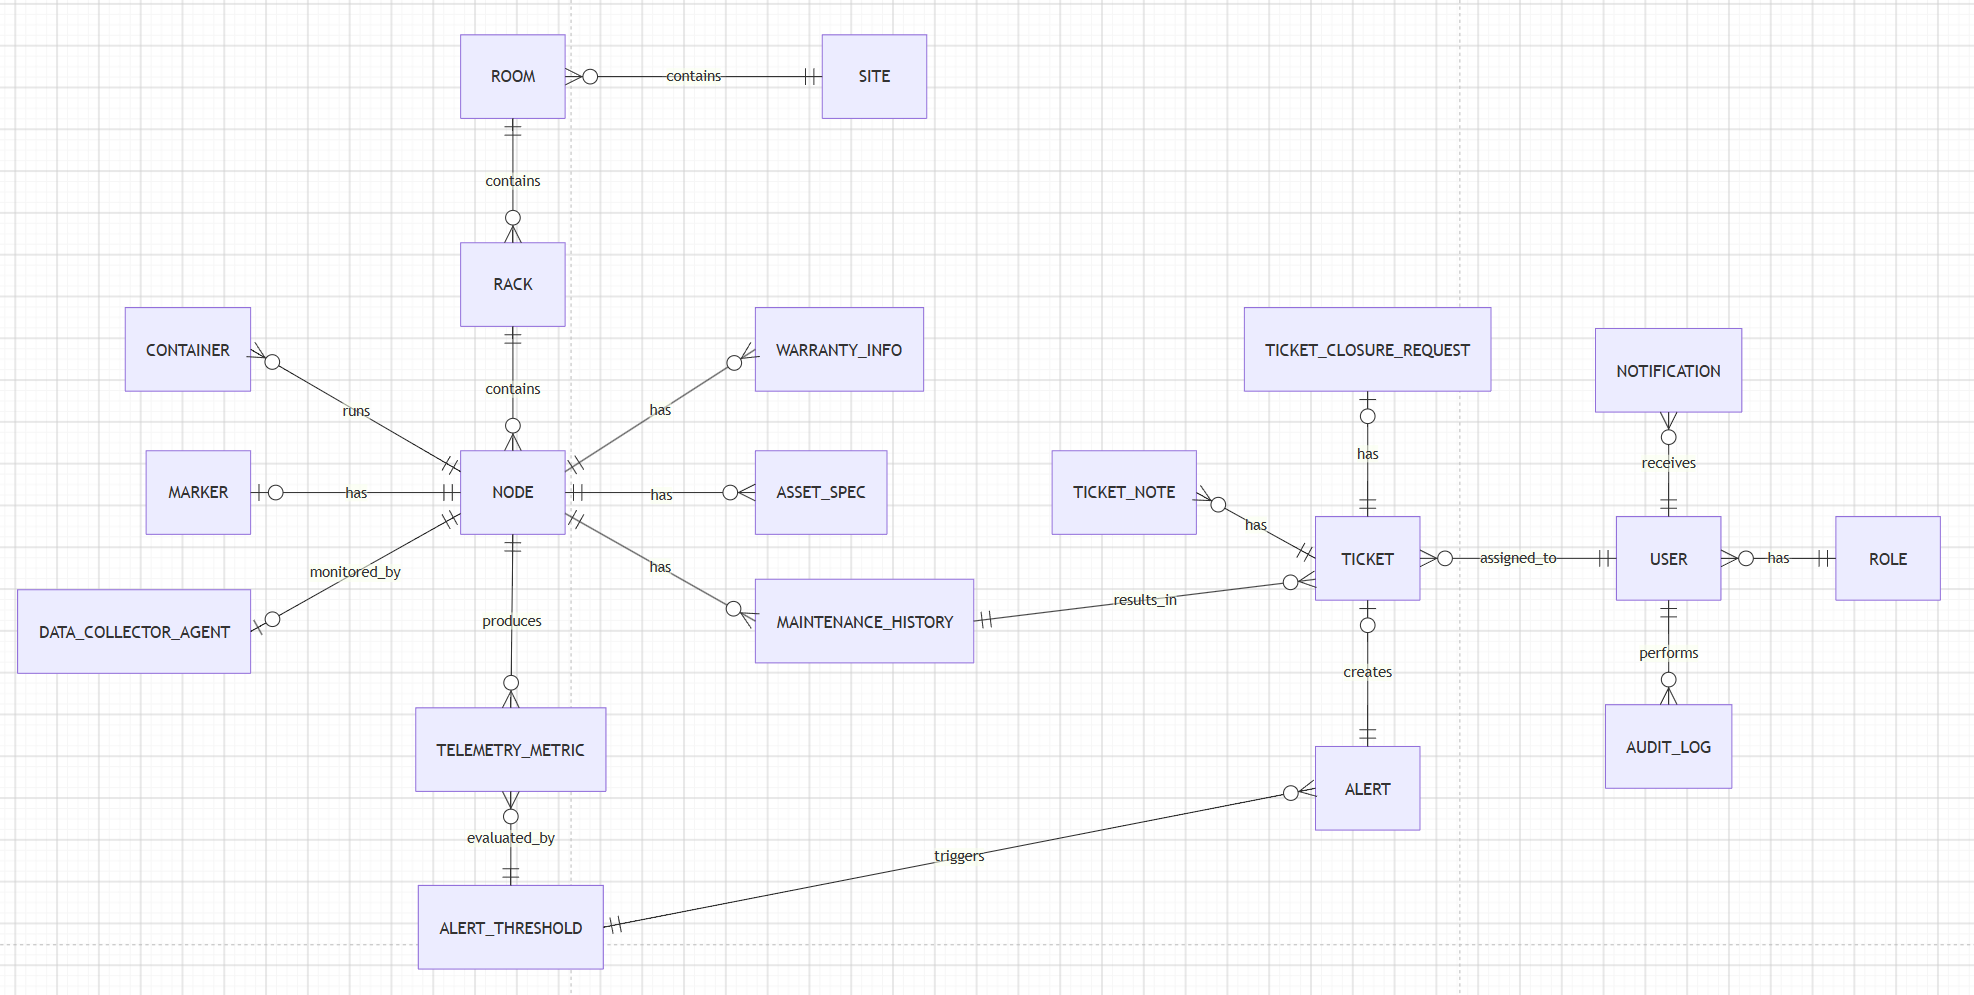
\includegraphics[width=0.98\textwidth]{ERD.png}
    \caption{Sơ đồ Thực thể - Mối quan hệ (ERD) hệ thống AR-IMMS}
    \label{fig:erd_diagram}
\end{figure}

\subsection{Phân tích các Thực thể chính (Entities)}
Hệ thống bao gồm 15 thực thể chính được nhóm thành 5 phân hệ dữ liệu cốt lõi:
\begin{enumerate}
    \item \textbf{Phân hệ Người dùng \& Kiểm toán:}
    \begin{itemize}
        \item \texttt{User}: Lưu trữ thông tin tài khoản, mật khẩu mã hóa (hash), vai trò RBAC (\textit{ADMINISTRATOR}, \textit{SYSTEM\_OPERATOR}, \textit{FIELD\_TECHNICIAN}) và họ tên.
        \item \texttt{AuditLog}: Ghi lại nhật ký tác động hệ thống bất biến (User ID, Thao tác, Loại tài nguyên, ID tài nguyên, Chi tiết JSON, IP Address, Timestamp).
    \end{itemize}
    \item \textbf{Phân hệ Cấu trúc Hạ tầng Digital Twin:}
    \begin{itemize}
        \item \texttt{Site}: Lưu thông tin các vị trí trung tâm dữ liệu (Mã, Tên, Địa điểm, Mô tả).
        \item \texttt{Room}: Lưu thông tin phòng máy thuộc Site (Mã, Tên, Tầng).
        \item \texttt{Rack}: Lưu thông tin tủ rack thuộc Room (Mã, Tên, Sức chứa Unit capacity, Năng lượng tối đa).
        \item \texttt{Node}: Lưu thông tin các máy chủ server thuộc Rack (Tên, Hostname, IP, MAC Address, Trạng thái ONLINE/OFFLINE/WARNING/CRITICAL, Vị trí U, Công suất tiêu thụ).
        \item \texttt{Container}: Lưu thông tin các workload/Docker container chạy trên Node (Container ID, Tên, Image, CPU\%, RAM usage, Trạng thái RUNNING/STOPPED, Số lần restart).
    \end{itemize}
    \item \textbf{Phân hệ Định danh AR \& Telemetry Agent:}
    \begin{itemize}
        \item \texttt{Marker}: Lưu mã định danh QR/ArUco Marker gán cho Node, loại marker và tọa độ không gian 3D dạng JSON.
        \item \texttt{DataCollectorAgent}: Lưu thông tin phần mềm Agent thu thập telemetry cài trên Node (Phiên bản, Trạng thái ACTIVE/INACTIVE, API Key Hash, Last Heartbeat).
        \item \texttt{TelemetryMetric}: CSDL chuỗi thời gian lưu dữ liệu đo đạc (CPU\%, RAM\%, Disk\%, Nhiệt độ, Network Rx/Tx, Timestamp).
    \end{itemize}
    \item \textbf{Phân hệ Cảnh báo, Sự cố \& Bảo trì:}
    \begin{itemize}
        \item \texttt{Alert}: Lưu cảnh báo bất thường từ Node (Loại chỉ số, Giá trị ngưỡng, Giá trị thực tế, Mức độ WARNING/CRITICAL, Trạng thái OPEN/ACKNOWLEDGED/RESOLVED/CLOSED, Số lần lặp lại occurrence count).
        \item \texttt{Ticket}: Lưu phiếu công việc bảo trì (Alert ID liên kết, Node ID, Tiêu đề, Mô tả, Mức ưu tiên LOW/MEDIUM/HIGH/CRITICAL, Trạng thái OPEN/ASSIGNED/IN\_PROGRESS/RESOLVED/CLOSED, ID người tạo, ID người được gán).
        \item \texttt{TicketNote}: Ghi chú diễn biến xử lý ticket từ kỹ thuật viên (Ticket ID, Author User ID, Nội dung ghi chú, Thời gian).
        \item \texttt{TicketClosureRequest}: Yêu cầu nghiệm thu đóng ticket từ Technician (Summary, Chi tiết xử lý, Trạng thái PENDING/APPROVED/REJECTED, ID người duyệt).
        \item \texttt{MaintenanceHistory}: Lịch sử bảo trì phục vụ kiểm toán thiết bị (Node ID, Ticket ID, Loại bảo trì, Mô tả, Người thực hiện, Thời gian).
    \end{itemize}
    \item \textbf{Phân hệ Thông số Kỹ thuật \& Bảo hành:}
    \begin{itemize}
        \item \texttt{AssetSpec}: Lưu cấu hình phần cứng chi tiết của Node (CPU Model, Cores, RAM GB, Storage GB, OS Name, OS Version).
        \item \texttt{WarrantyInfo}: Lưu thông tin bảo hành máy chủ (Vendor, Model Number, Serial Number, Ngày mua, Ngày bắt đầu/kết thúc bảo hành, Đơn vị hỗ trợ).
    \end{itemize}
\end{enumerate}

\subsection{Phân tích Mối quan hệ giữa các Thực thể (Entity Relationships)}
Bảng dưới đây tổng hợp bản chất mối quan hệ, khóa ngoại (Foreign Key) và quy tắc ràng buộc giữa các thực thể:

\begin{longtable}{|p{3cm}|p{3cm}|p{2.5cm}|p{5cm}|}
\hline
\textbf{Thực thể Cha} & \textbf{Thực thể Con} & \textbf{Tỷ lệ (Card.)} & \textbf{Khóa ngoại (FK) \& Diễn giải} \\ \hline
\endhead
\texttt{Site} & \texttt{Room} & $1 : N$ & \texttt{Room.site\_id} $\rightarrow$ Một Site chứa nhiều Room. \\ \hline
\texttt{Room} & \texttt{Rack} & $1 : N$ & \texttt{Rack.room\_id} $\rightarrow$ Một Room chứa nhiều tủ Rack. \\ \hline
\texttt{Rack} & \texttt{Node} & $1 : N$ & \texttt{Node.rack\_id} $\rightarrow$ Một Rack chứa nhiều máy chủ Node. \\ \hline
\texttt{Node} & \texttt{Container} & $1 : N$ & \texttt{Container.node\_id} $\rightarrow$ Một Node chạy nhiều Container workload. \\ \hline
\texttt{Node} & \texttt{Marker} & $1 : N$ & \texttt{Marker.node\_id} $\rightarrow$ Một Node có các mã AR Marker định danh. \\ \hline
\texttt{Node} & \texttt{DataCollectorAgent} & $1 : N$ & \texttt{DataCollectorAgent.node\_id} $\rightarrow$ Một Node cài Agent thu thập. \\ \hline
\texttt{Node} & \texttt{TelemetryMetric} & $1 : N$ & \texttt{TelemetryMetric.node\_id} $\rightarrow$ Lưu chuỗi bản tin telemetry. \\ \hline
\texttt{Node} & \texttt{Alert} & $1 : N$ & \texttt{Alert.node\_id} $\rightarrow$ Phát sinh các cảnh báo cho Node. \\ \hline
\texttt{Alert} & \texttt{Ticket} & $0..1 : N$ & \texttt{Ticket.alert\_id} $\rightarrow$ Chuyển đổi cảnh báo thành Ticket. \\ \hline
\texttt{Node} & \texttt{Ticket} & $1 : N$ & \texttt{Ticket.node\_id} $\rightarrow$ Ticket gắn liền với thiết bị mục tiêu. \\ \hline
\texttt{User} & \texttt{Ticket} & $1 : N$ & \texttt{Ticket.created\_by\_user\_id}, \texttt{assigned\_to\_user\_id}. \\ \hline
\texttt{Ticket} & \texttt{TicketNote} & $1 : N$ & \texttt{TicketNote.ticket\_id} $\rightarrow$ Các ghi chú xử lý công việc. \\ \hline
\texttt{Ticket} & \texttt{TicketClosureRequest} & $1 : 0..1$ & \texttt{TicketClosureRequest.ticket\_id} $\rightarrow$ Yêu cầu đóng ticket. \\ \hline
\texttt{Node} & \texttt{MaintenanceHistory} & $1 : N$ & \texttt{MaintenanceHistory.node\_id} $\rightarrow$ Nhật ký lịch sử bảo trì. \\ \hline
\texttt{Node} & \texttt{AssetSpec} & $1 : 1$ & \texttt{AssetSpec.node\_id} $\rightarrow$ Thông số phần cứng chi tiết Node. \\ \hline
\texttt{Node} & \texttt{WarrantyInfo} & $1 : 1$ & \texttt{WarrantyInfo.node\_id} $\rightarrow$ Hồ sơ bảo hành thiết bị. \\ \hline
\texttt{User} & \texttt{AuditLog} & $1 : N$ & \texttt{AuditLog.user\_id} $\rightarrow$ Nhật ký kiểm toán thao tác người dùng. \\ \hline
\end{longtable}


\chapter{QUY TRÌNH NGHIỆP VỤ}

\section{Tổng quan luồng vận hành hệ thống}
Quy trình dịch vụ của hệ thống AR-IMMS hoạt động theo mô hình khép kín (Closed-loop Workflow) gồm 5 giai đoạn liên tục để đảm bảo mọi sự cố từ khi phát sinh cho đến khi hoàn thành sửa chữa đều được theo dõi và ghi nhật ký minh bạch.

\begin{figure}[H]
\centering
\textbf{[1. Thu thập \& Giám sát]} $\longrightarrow$ \textbf{[2. Phát hiện \& Cảnh báo]} $\longrightarrow$ \textbf{[3. Phân công Ticket]} $\longrightarrow$ \textbf{[4. Xử lý bằng AR]} $\longrightarrow$ \textbf{[5. Nghiệm thu \& Kiểm toán]}
\caption{Sơ đồ luồng vận hành khép kín 5 giai đoạn của AR-IMMS}
\end{figure}

\section{Phân tích chi tiết 5 giai đoạn quy trình}

\subsection{Giai đoạn 1: Thu thập Dữ liệu \& Giám sát (Data Collection \& Monitoring)}
\begin{itemize}
    \item \textbf{Tác nhân tham gia:} Monitoring Agent (Tự động), System Operator, Digital Twin Engine.
    \item \textbf{Mô tả chi tiết:}
    \begin{enumerate}
        \item \textbf{Thu thập tự động:} Monitoring Agent được cài đặt trên từng máy chủ trong Mini Data Center Testbed tự động đọc thông số phần cứng (CPU, RAM, Nhiệt độ, Disk, Network) và thông tin Docker container. Dữ liệu được đóng gói thành các chuỗi JSON telemetry và truyền về Backend API qua kết nối mTLS / WebSocket theo chu kỳ định sẵn (mặc định 5 giây/lần).
        \item \textbf{Cập nhật giao diện \& Digital Twin:} Backend API tiếp nhận dữ liệu, lưu vào cơ sở dữ liệu chuỗi thời gian (Time-series Data) và thực hiện phát dòng (broadcast) qua WebSocket Gateway tới Web Command Center. Giao diện bảng điều khiển và cây phân cấp Digital Twin ($\text{Site} \rightarrow \text{Room} \rightarrow \text{Rack} \rightarrow \text{Server} \rightarrow \text{Workload}$) lập tức cập nhật chỉ số biểu đồ và màu sắc trạng thái.
        \item \textbf{Giám sát kết nối ngầm:} Hệ thống chạy một tiến trình kiểm tra (Heartbeat Monitor). Nếu vượt quá 90 giây liên tục không nhận được bất kỳ dữ liệu telemetry nào từ một Agent, hệ thống tự động chuyển trạng thái của Server đó sang \textit{Unavailable} (Mất kết nối).
    \end{enumerate}
\end{itemize}

\subsection{Giai đoạn 2: Phát hiện Sự cố \& Phát Cảnh báo (Incident Detection \& Alerting)}
\begin{itemize}
    \item \textbf{Tác nhân tham gia:} Automated Monitoring Engine, System Operator.
    \item \textbf{Mô tả chi tiết:}
    \begin{enumerate}
        \item \textbf{So sánh ngưỡng tự động:} Ngay khi nhận được bản tin telemetry, Monitoring Engine tiến hành so sánh chỉ số với bảng quy tắc ngưỡng (ví dụ: CPU usage $> 90\%$, Nhiệt độ $> 75^\circ\text{C}$).
        \item \textbf{Tạo Alert \& Khử trùng lặp:} Khi phát hiện chỉ số bất thường, hệ thống tự động khởi tạo bản ghi Cảnh báo mới ở trạng thái \textit{Open}. Nếu điều kiện bất thường kéo dài qua nhiều chu kỳ gửi dữ liệu, thuật toán khử trùng lặp (Alert Storm Suppression) sẽ gộp các sự cố trùng vào cảnh báo đang tồn tại thay vì tạo hàng loạt bản ghi mới.
        \item \textbf{Hiển thị vị trí không gian:} Cảnh báo được làm nổi bật bằng mã màu quy ước (Vàng: Warning, Đỏ: Critical) trên Web Dashboard và phát sáng nhấp nháy tại vị trí tương ứng trên mô hình Digital Twin.
        \item \textbf{Xác nhận tiếp nhận:} Chuyên viên vận hành (System Operator) quan sát được cảnh báo trên màn hình chỉ huy và nhấn nút \textbf{Xác nhận (Acknowledge)} để ghi nhận hệ thống đang xem xét sự cố. Trạng thái Alert chuyển thành \textit{Acknowledged}.
    \end{enumerate}
\end{itemize}

\subsection{Giai đoạn 3: Quản lý \& Phân công Phiếu Hỗ trợ (Ticket Creation \& Assignment)}
\begin{itemize}
    \item \textbf{Tác nhân tham gia:} System Operator, Field Technician.
    \item \textbf{Mô tả chi tiết:}
    \begin{enumerate}
        \item \textbf{Khởi tạo Ticket bảo trì:} Từ cảnh báo đã được xác nhận (hoặc qua yêu cầu bảo trì định kỳ), Operator chọn chức năng "Tạo Ticket". Hệ thống tự động trích xuất các thông tin ngữ cảnh: Mã máy chủ, Vị trí phòng/rack, Loại lỗi, Thời gian phát sinh và Chỉ số telemetry tại thời điểm bị lỗi vào nội dung Ticket.
        \item \textbf{Phân công nhân sự:} Operator lựa chọn Kỹ thuật viên hiện trường (Field Technician) đang trong ca trực và nhấn "Giao việc". Trạng thái Ticket chuyển thành \textit{Assigned}.
        \item \textbf{Tiếp nhận thông báo di động:} Kỹ thuật viên nhận được thông báo đẩy (Push Notification) trên ứng dụng di động AR. Kỹ thuật viên mở app để xem danh sách nhiệm vụ, vị trí chính xác của tủ Rack và Server cần kiểm tra.
    \end{enumerate}
\end{itemize}

\subsection{Giai đoạn 4: Xử lý Sự cố Tại chỗ bằng AR (On-site AR Field Maintenance)}
\begin{itemize}
    \item \textbf{Tác nhân tham gia:} Field Technician, Mobile AR Application, Backend API.
    \item \textbf{Mô tả chi tiết:}
    \begin{enumerate}
        \item \textbf{Định vị \& Quét thiết bị:} Kỹ thuật viên di chuyển tới phòng máy chủ, tìm đến vị trí tủ Rack và sử dụng ứng dụng di động AR để quét mã QR / ArUco Marker được dán phía trước máy chủ.
        \item \textbf{Hiển thị lớp phủ AR (AR Overlay):} Ứng dụng di động nhận diện mã marker, truy vấn dữ liệu từ Backend API và hiển thị ngay trên màn hình camera các thẻ thông tin kỹ thuật số bao gồm: Tên thiết bị, Chỉ số CPU/RAM/Temp thời gian thực, Danh sách container/workload đang chạy và thông tin cảnh báo active.
        \item \textbf{Thực hiện thao tác \& Xác thực 2 bước (Step-up Verification):} Kỹ thuật viên thực hiện kiểm tra phần cứng, cắm lại cáp hoặc thực hiện thao tác can thiệp dịch vụ (ví dụ: Khởi động lại container). Nếu thực hiện thao tác can thiệp có tính rủi ro trên ứng dụng AR, ứng dụng sẽ yêu cầu xác thực 2 bước để phòng ngừa bấm nhầm.
        \item \textbf{Ghi nhận nguyên nhân \& Tiến độ:} Kỹ thuật viên nhập ghi chú chẩn đoán, nguyên nhân sự cố và kết quả sửa chữa trực tiếp trên ứng dụng di động. Trạng thái Ticket chuyển thành \textit{In-Progress}.
    \end{enumerate}
\end{itemize}

\subsection{Giai đoạn 5: Đóng Sự cố \& Kiểm toán Hệ thống (Resolution \& Audit Trail)}
\begin{itemize}
    \item \textbf{Tác nhân tham gia:} Field Technician, System Operator, Audit Log Module.
    \item \textbf{Mô tả chi tiết:}
    \begin{enumerate}
        \item \textbf{Yêu cầu đóng Ticket:} Sau khi khắc phục xong sự cố tại chỗ, Kỹ thuật viên đánh dấu công việc hoàn thành trên app AR và nhấn \textbf{Gửi yêu cầu đóng Ticket (Closure Request)}. Trạng thái Ticket chuyển thành \textit{Resolved}.
        \item \textbf{Nghiệm thu \& Phê duyệt:} System Operator kiểm tra lại chỉ số telemetry thời gian thực của máy chủ đó trên Web Command Center. Khi xác nhận thông số đã trở về ngưỡng an toàn (màu xanh), Operator nhấn nút \textbf{Phê duyệt đóng Ticket}. Trạng thái Ticket và Alert chính thức chuyển thành \textit{Closed}.
        \item \textbf{Ghi nhật ký kiểm toán bất biến (Immutable Audit Log):} Toàn bộ mốc thời gian, dữ liệu telemetry tại thời điểm sự cố, danh tính người tiếp nhận, nhật ký quét AR và các hành động khắc phục được tự động lưu trữ vĩnh viễn vào Audit Trail của hệ thống, phục vụ công tác truy vết và lập báo cáo thống kê PUE.
    \end{enumerate}
\end{itemize}

\section{Bảng ma trận phân vùng trách nhiệm (RACI Matrix)}
Bảng dưới đây mô tả sự phân công trách nhiệm giữa các bên đối với từng hành động chính trong quy trình dịch vụ:
\begin{itemize}
    \item \textbf{R (Responsible):} Người trực tiếp thực hiện công việc.
    \item \textbf{A (Accountable):} Người chịu trách nhiệm phê duyệt cuối cùng.
    \item \textbf{C (Consulted):} Người cung cấp thông tin/tư vấn.
    \item \textbf{I (Informed):} Người nhận thông báo kết quả.
\end{itemize}

\begin{table}[H]
\centering
\begin{tabularx}{\textwidth}{|X|c|c|c|c|}
\hline
\textbf{Giai đoạn / Hành động nghiệp vụ} & \textbf{Admin} & \textbf{Operator} & \textbf{Technician} & \textbf{Agent (Auto)} \\ \hline
Thu thập Telemetry \& Kiểm tra Heartbeat & I & I & - & R / A \\ \hline
Cấu hình ngưỡng cảnh báo hệ thống & A & R & C & - \\ \hline
Phát hiện vượt ngưỡng \& Khởi tạo Alert & I & I & - & R / A \\ \hline
Xác nhận Alert (Acknowledge) & I & R / A & I & - \\ \hline
Tạo phiếu Ticket \& Phân công nhân sự & I & R / A & I & - \\ \hline
Quét mã AR, kiểm tra & I & I & R / A & - \\ \hline
Thực hiện thao tác sửa chữa & I & I & R / A & - \\ \hline
Nghiệm thu \& Phê duyệt đóng Ticket & I & R / A & C & - \\ \hline
Ghi nhật ký kiểm toán Audit Log & I & I & I & R / A \\ \hline
\end{tabularx}
\caption{Ma trận phân công trách nhiệm RACI cho quy trình vận hành AR-IMMS}
\end{table}


\chapter{YÊU CẦU CHỨC NĂNG}

Chương này đặc tả danh mục đầy đủ các yêu cầu chức năng (\textit{Functional Requirements - FR}) của hệ thống AR-IMMS từ FR-01 đến FR-32, phân chia chi tiết theo 10 phân hệ nghiệp vụ phần mềm.

\section{Phân hệ 1: Xác thực và Phân quyền (Authentication \& RBAC)}
\begin{longtable}{|p{2.5cm}|p{4cm}|p{8cm}|}
\hline
\textbf{Mã YCKT} & \textbf{Tên chức năng} & \textbf{Mô tả yêu cầu chi tiết} \\ \hline
\endhead
\textbf{FR-01} & Đăng nhập hệ thống & Hệ thống cho phép người dùng (Admin, Operator, Technician) đăng nhập bằng tài khoản và mật khẩu. Sau khi xác thực thành công, hệ thống cấp phát JSON Web Token (JWT) và định tuyến đến giao diện tương ứng với vai trò. \\ \hline
\textbf{FR-02} & Quản lý phiên làm việc \& Đăng xuất & Hệ thống hỗ trợ đăng xuất, hủy JWT token hiện tại và tự động ngắt phiên làm việc sau một khoảng thời gian không hoạt động (Inactivity Timeout). \\ \hline
\textbf{FR-03} & Phân quyền truy cập dựa trên vai trò (RBAC) & Hệ thống kiểm soát quyền truy cập tài nguyên API và chức năng UI theo vai trò: Administrator có toàn quyền; Operator có quyền quản lý vận hành, tài sản, ticket; Technician có quyền tiếp nhận ticket và sử dụng ứng dụng AR. \\ \hline
\textbf{FR-04} & Quản lý tài khoản người dùng & Cho phép Administrator khởi tạo tài khoản mới, cập nhật thông tin cá nhân, gán/thay đổi vai trò, đặt lại mật khẩu và khóa/mở khóa tài khoản. \\ \hline
\end{longtable}

\section{Phân hệ 2: Quản lý Cơ sở hạ tầng Phân cấp (Infrastructure Management)}
\begin{longtable}{|p{2.5cm}|p{4cm}|p{8cm}|}
\hline
\textbf{Mã YCKT} & \textbf{Tên chức năng} & \textbf{Mô tả yêu cầu chi tiết} \\ \hline
\endhead
\textbf{FR-05} & Quản lý Site \& Room & Cho phép Operator khởi tạo, chỉnh sửa, xóa và truy vấn thông tin các vị trí trung tâm dữ liệu (Site) và các phòng chứa máy chủ (Room). \\ \hline
\textbf{FR-06} & Quản lý tủ Rack & Cho phép Operator thêm mới tủ Rack vào phòng máy, khai báo thông số chiều cao (U-size), vị trí tọa độ trong phòng và sức chứa tối đa. \\ \hline
\textbf{FR-07} & Quản lý Server/Node & Cho phép Operator đăng ký nút máy chủ mới, khai báo vị trí số U trong tủ Rack, thông số phần cứng (CPU cores, RAM size, Disk capacity, IP address). \\ \hline
\textbf{FR-08} & Quản lý Container/Workload & Cho phép hệ thống ghi nhận các ứng dụng, dịch vụ hoặc Docker container đang vận hành trên từng nút máy chủ. \\ \hline
\textbf{FR-09} & Ánh xạ QR/ArUco Marker & Cho phép Operator tạo mã định danh duy nhất và liên kết thông tin mã QR/ArUco Marker với nút máy chủ vật lý tương ứng phục vụ quét nhận diện trên app AR. \\ \hline
\end{longtable}

\section{Phân hệ 3: Giám sát và Thu thập Telemetry (Telemetry Monitoring)}
\begin{longtable}{|p{2.5cm}|p{4cm}|p{8cm}|}
\hline
\textbf{Mã YCKT} & \textbf{Tên chức năng} & \textbf{Mô tả yêu cầu chi tiết} \\ \hline
\endhead
\textbf{FR-10} & Thu thập dữ liệu Telemetry & Monitoring Agent tự động thu thập thông số CPU, RAM, Nhiệt độ, Disk, Network và trạng thái Docker container từ máy chủ, gửi về Backend API qua mTLS/WebSocket theo chu kỳ mặc định 5 giây. \\ \hline
\textbf{FR-11} & Phát dòng dữ liệu thời gian thực & Backend API chuyển tiếp dữ liệu telemetry tới Web Command Center qua kết nối WebSocket/Socket.IO để vẽ đồ thị diễn biến thời gian thực mà không cần tải lại trang. \\ \hline
\textbf{FR-12} & Lưu trữ dữ liệu lịch sử Telemetry & Hệ thống lưu trữ các bản ghi telemetry thu thập được vào CSDL chuỗi thời gian (Time-series DB) phục vụ việc tra cứu diễn biến trong quá khứ và lập báo cáo. \\ \hline
\textbf{FR-13} & Phát hiện ngắt kết nối Agent & Hệ thống tự động theo dõi kết nối Agent. Nếu quá 90 giây không nhận được telemetry từ một máy chủ, hệ thống cập nhật trạng thái máy chủ đó thành Unavailable và phát cảnh báo mất kết nối. \\ \hline
\end{longtable}

\section{Phân hệ 4: Mô hình số Digital Twin (Digital Twin Engine)}
\begin{longtable}{|p{2.5cm}|p{4cm}|p{8cm}|}
\hline
\textbf{Mã YCKT} & \textbf{Tên chức năng} & \textbf{Mô tả yêu cầu chi tiết} \\ \hline
\endhead
\textbf{FR-14} & Trực quan hóa cây cấu trúc Digital Twin & Cho phép hiển thị mô hình cây tài sản 3D/2D tương tác theo cấu trúc phân cấp: Site $\rightarrow$ Room $\rightarrow$ Rack $\rightarrow$ Server $\rightarrow$ Workload. \\ \hline
\textbf{FR-15} & Đồng bộ trạng thái kỹ thuật số & Hệ thống cập nhật màu sắc hiển thị của thiết bị trên Digital Twin tương ứng với trạng thái vận hành thời gian thực (Xanh: Healthy, Vàng: Warning, Đỏ: Critical, Xám: Unavailable). \\ \hline
\textbf{FR-16} & Khoan sâu dữ liệu (Drill-down Navigation) & Hỗ trợ thao tác nhấp chuột "3-click drill-down" từ mức tổng quan toàn Site xuống phòng máy, tủ Rack, từng máy chủ và đến từng log container đang chạy. \\ \hline
\end{longtable}

\section{Phân hệ 5: Quản lý Cảnh báo (Alert Management)}
\begin{longtable}{|p{2.5cm}|p{4cm}|p{8cm}|}
\hline
\textbf{Mã YCKT} & \textbf{Tên chức năng} & \textbf{Mô tả yêu cầu chi tiết} \\ \hline
\endhead
\textbf{FR-17} & Cấu hình ngưỡng cảnh báo & Cho phép Operator thiết lập và thay đổi các ngưỡng cảnh báo cho từng chỉ số (ví dụ: CPU Warning $> 80\%$, CPU Critical $> 90\%$, Nhiệt độ $> 75^\circ\text{C}$). \\ \hline
\textbf{FR-18} & Tự động sinh Cảnh báo & Hệ thống tự động khởi tạo bản ghi Alert mới ở trạng thái \textit{Open} ngay khi phát hiện chỉ số thu thập vượt ngưỡng cấu hình hoặc mất kết nối. \\ \hline
\textbf{FR-19} & Lọc trùng lặp cảnh báo (Alert Suppression) & Hệ thống áp dụng thuật toán khử trùng lặp để ngăn chặn hiện tượng "bão cảnh báo" (Alert Storm), gộp các bất thường liên tục trên cùng thiết bị vào 1 Alert duy nhất. \\ \hline
\textbf{FR-20} & Quản lý vòng đời Alert & Cho phép Operator xem danh sách Alert, nhấn nút Xác nhận (Acknowledge), cập nhật trạng thái thành Resolved hoặc Closed khi sự cố đã được khắc phục. \\ \hline
\end{longtable}

\section{Phân hệ 6: Quản lý Sự cố (Incident Management)}
\begin{longtable}{|p{2.5cm}|p{4cm}|p{8cm}|}
\hline
\textbf{Mã YCKT} & \textbf{Tên chức năng} & \textbf{Mô tả yêu cầu chi tiết} \\ \hline
\endhead
\textbf{FR-21} & Chuyển đổi Alert thành Incident & Cho phép Operator khởi tạo một bản ghi Sự cố (Incident) từ một Alert đang hoạt động, tự động kế thừa toàn bộ thông tin mã máy chủ, vị trí và mức độ nghiêm trọng. \\ \hline
\textbf{FR-22} & Phân loại \& Đánh giá mức độ ưu tiên & Cho phép thiết lập mức độ ưu tiên xử lý sự cố (Low, Medium, High, Critical) và gán thời gian cam kết khắc phục (SLA). \\ \hline
\textbf{FR-23} & Theo dõi tiến độ giải quyết Incident & Cho phép người quản lý theo dõi toàn bộ quá trình xử lý sự cố từ lúc phát sinh, phân công cho đến khi kiểm tra nghiệm thu hoàn thành. \\ \hline
\end{longtable}

\section{Phân hệ 7: Quản lý Bảo trì (Ticket Management)}
\begin{longtable}{|p{2.5cm}|p{4cm}|p{8cm}|}
\hline
\textbf{Mã YCKT} & \textbf{Tên chức năng} & \textbf{Mô tả yêu cầu chi tiết} \\ \hline
\endhead
\textbf{FR-24} & Khởi tạo phiếu Ticket bảo trì & Cho phép Operator tạo Ticket xử lý sự cố hoặc Ticket bảo trì định kỳ, điền mô tả công việc, đính kèm tài liệu hướng dẫn và chọn thiết bị mục tiêu. \\ \hline
\textbf{FR-25} & Phân công Ticket cho Kỹ thuật viên & Cho phép Operator giao Ticket cho Kỹ thuật viên hiện trường. Hệ thống tự động gửi thông báo đẩy tới ứng dụng di động của Kỹ thuật viên đó. \\ \hline
\textbf{FR-26} & Cập nhật tiến độ \& Yêu cầu đóng Ticket & Cho phép Technician cập nhật trạng thái công việc (In-Progress, Resolved), ghi nhận nguyên nhân, hành động khắc phục và gửi yêu cầu phê duyệt đóng Ticket tới Operator. \\ \hline
\end{longtable}

\section{Phân hệ 8: Quản lý Tài sản và Bảo hành (Asset Lifecycle)}
\begin{longtable}{|p{2.5cm}|p{4cm}|p{8cm}|}
\hline
\textbf{Mã YCKT} & \textbf{Tên chức năng} & \textbf{Mô tả yêu cầu chi tiết} \\ \hline
\endhead
\textbf{FR-27} & Quản lý thông tin bảo hành & Cho phép lưu trữ và tra cứu nhà cung cấp, ngày mua, thời hạn bảo hành, hợp đồng dịch vụ đi kèm của từng máy chủ và thiết bị hạ tầng. \\ \hline
\textbf{FR-28} & Quản lý lịch sử thay thế linh kiện & Cho phép ghi nhận nhật ký thay thế, nâng cấp linh kiện (RAM, CPU, Hard Drive, PSU) của từng thiết bị trong suốt vòng đời vận hành. \\ \hline
\end{longtable}

\section{Phân hệ 9: Ứng dụng Thực tế Tăng cường (Mobile AR Application)}
\begin{longtable}{|p{2.5cm}|p{4cm}|p{8cm}|}
\hline
\textbf{Mã YCKT} & \textbf{Tên chức năng} & \textbf{Mô tả yêu cầu chi tiết} \\ \hline
\endhead
\textbf{FR-29} & Quét nhận diện QR/ArUco Marker & Ứng dụng AR trên thiết bị di động sử dụng camera để quét mã QR hoặc ArUco Marker gắn trên vỏ máy chủ vật lý, nhận diện chính xác ID thiết bị trong thời gian $< 1$ giây. \\ \hline
\textbf{FR-30} & Hiển thị thông tin lớp phủ AR (Overlay) & Sau khi nhận diện thiết bị, app hiển thị lớp phủ dữ liệu ảo (AR Overlay) bao gồm: Tên máy chủ, chỉ số CPU/RAM/Temp trực tiếp, các cảnh báo active và log dịch vụ tương ứng. \\ \hline
\end{longtable}

\section{Phân hệ 10: Báo cáo và Nhật ký Kiểm toán (Reporting \& Audit Trail)}
\begin{longtable}{|p{2.5cm}|p{4cm}|p{8cm}|}
\hline
\textbf{Mã YCKT} & \textbf{Tên chức năng} & \textbf{Mô tả yêu cầu chi tiết} \\ \hline
\endhead
\textbf{FR-31} & Thống kê \& Báo cáo vận hành & Cho phép tạo và xuất các báo cáo định kỳ về tình hình telemetry, số lượng sự cố, chỉ số MTTR và hiệu năng PUE dưới dạng PDF hoặc Excel. \\ \hline
\textbf{FR-32} & Ghi nhật ký kiểm toán (Audit Trail) & Hệ thống tự động ghi lại tất cả các hành động tác động hệ thống (thay đổi cấu hình, tạo/duyệt ticket, xác thực AR) thành bản ghi Audit Log bất biến không thể sửa xóa. \\ \hline
\end{longtable}


\chapter{ĐẶC TẢ USE CASE}

Chương này trình bày chi tiết về các tác nhân, biểu đồ Use Case tổng quát, danh mục 26 Use Case và đặc tả chi tiết cho từng Use Case trong hệ thống AR-IMMS.

\section{Danh sách Tác nhân (Actors)}
\begin{enumerate}
    \item \textbf{Quản trị viên (Administrator):} Người có quyền hạn cao nhất, thực hiện quản lý người dùng, phân quyền, cấu hình hệ thống, thiết lập ngưỡng cảnh báo và xem nhật ký kiểm toán.
    \item \textbf{Chuyên viên Vận hành (System Operator):} Người trực tiếp vận hành hạ tầng hằng ngày, quản lý tài sản, theo dõi bảng điều khiển giám sát, xử lý cảnh báo, tạo và phân công ticket bảo trì, duyệt đóng ticket và xem báo cáo.
    \item \textbf{Kỹ thuật viên hiện trường (Field Technician):} Người làm việc tại hiện trường phòng máy chủ, tiếp nhận ticket, sử dụng ứng dụng di động AR để quét nhận diện thiết bị, xem telemetry trực tiếp, thực hiện sửa chữa và gửi yêu cầu đóng ticket.
    \item \textbf{Monitoring Agent / IoT Engine:} Tác nhân hệ thống tự động thu thập dữ liệu telemetry từ máy chủ và phát cảnh báo tự động.
\end{enumerate}

\section{Biểu đồ Use Case tổng quát}
Sơ đồ Use Case tổng quan được chia thành 7 phân nhóm nghiệp vụ: Xác thực, Quản lý tài sản, Giám sát, Cảnh báo, Quản lý Ticket, Thực tế tăng cường (AR) và Báo cáo.

\section{Danh mục Use Case tổng hợp (UC-01 đến UC-26)}
\begin{longtable}{|p{1.5cm}|p{4.5cm}|p{3.5cm}|p{5cm}|}
\hline
\textbf{Mã UC} & \textbf{Tên Use Case} & \textbf{Tác nhân chính} & \textbf{Mô tả ngắn gọn} \\ \hline
\endhead
\multicolumn{4}{|l|}{\textbf{1. Phân hệ Xác thực (Authentication)}} \\ \hline
UC-01 & Đăng nhập & Admin, Operator, Tech & Nhập tài khoản/mật khẩu để lấy JWT Token. \\ \hline
UC-02 & Đăng xuất & Admin, Operator, Tech & Hủy phiên làm việc hiện tại. \\ \hline
UC-03 & Đặt lại mật khẩu & Admin, Operator, Tech & Khôi phục lại mật khẩu khi quên. \\ \hline
UC-04 & Quản lý tài khoản & Administrator & Tạo, sửa, phân quyền, khóa tài khoản. \\ \hline
\multicolumn{4}{|l|}{\textbf{2. Phân hệ Quản lý tài sản (Asset Management)}} \\ \hline
UC-05 & Thêm tài sản/máy chủ & System Operator & Khai báo máy chủ, rack, vị trí không gian. \\ \hline
UC-06 & Cập nhật tài sản & System Operator & Chỉnh sửa cấu hình, thông số máy chủ. \\ \hline
UC-07 & Xóa tài sản & System Operator & Vô hiệu hóa tài sản khỏi hệ thống. \\ \hline
UC-08 & Xem danh sách tài sản & Operator, Technician & Tra cứu, lọc danh sách tài sản. \\ \hline
UC-09 & Quản lý ánh xạ AR Marker & System Operator & Gán mã QR/ArUco cho máy chủ. \\ \hline
\multicolumn{4}{|l|}{\textbf{3. Phân hệ Giám sát (Monitoring)}} \\ \hline
UC-10 & Xem Dashboard giám sát & Operator, Admin & Màn hình telemetry thời gian thực. \\ \hline
UC-11 & Xem chi tiết Server & Operator, Technician & Mức CPU, RAM, Temp, Docker stats. \\ \hline
UC-12 & Cấu hình ngưỡng cảnh báo & System Operator, Admin & Đặt giá trị ngưỡng Warning/Critical. \\ \hline
\multicolumn{4}{|l|}{\textbf{4. Phân hệ Cảnh báo (Alert)}} \\ \hline
UC-13 & Nhận thông báo Cảnh báo & Operator, Technician & Nhận thông báo khi chỉ số vượt ngưỡng. \\ \hline
UC-14 & Xem danh sách cảnh báo & Operator, Technician & Truy vấn lịch sử Alert. \\ \hline
UC-15 & Xác nhận Cảnh báo & System Operator & Chuyển trạng thái Alert thành Acknowledged. \\ \hline
UC-16 & Xử lý \& Đóng cảnh báo & System Operator & Đóng Alert khi thông số an toàn. \\ \hline
\multicolumn{4}{|l|}{\textbf{5. Phân hệ Quản lý Ticket (Ticket Management)}} \\ \hline
UC-17 & Khởi tạo Ticket & System Operator & Tạo phiếu bảo trì từ Alert. \\ \hline
UC-18 & Gán Ticket cho Kỹ thuật viên & System Operator & Phân công nhiệm vụ sửa chữa. \\ \hline
UC-19 & Cập nhật trạng thái Ticket & Field Technician & Ghi nhận tiến độ In-Progress/Resolved. \\ \hline
UC-20 & Xem lịch sử Ticket & Admin, Operator, Tech & Tra cứu hồ sơ bảo trì thiết bị. \\ \hline
\multicolumn{4}{|l|}{\textbf{6. Phân hệ Thực tế tăng cường (AR)}} \\ \hline
UC-21 & Quét \& Xem AR Overlay & Field Technician & Xem telemetry trực tiếp trên vỏ máy chủ. \\ \hline
UC-22 & Điều hướng AR trong phòng & Field Technician & Dẫn đường trực quan tới vị trí tủ Rack. \\ \hline
UC-23 & Xác thực thao tác nguy hiểm & Field Technician & Step-up verification trên app AR. \\ \hline
\multicolumn{4}{|l|}{\textbf{7. Phân hệ Báo cáo (Report)}} \\ \hline
UC-24 & Lập báo cáo vận hành & Operator, Admin & Tổng hợp chỉ số MTTR, sự cố, PUE. \\ \hline
UC-25 & Xuất báo cáo PDF/Excel & Operator, Admin & Xuất báo cáo ra định dạng file. \\ \hline
UC-26 & Xem nhật ký Audit Log & Administrator & Tra cứu nhật ký tác động hệ thống. \\ \hline
\end{longtable}

\section{Đặc tả chi tiết các Use Case trọng tâm}

\subsection{Đặc tả UC-01: Đăng nhập hệ thống}
\begin{table}[H]
\centering
\begin{tabular}{|p{4cm}|p{10.5cm}|}
\hline
\textbf{Mã Use Case} & \textbf{UC-01} \\ \hline
\textbf{Tên Use Case} & Đăng nhập hệ thống \\ \hline
\textbf{Tác nhân} & Administrator, System Operator, Field Technician \\ \hline
\textbf{Mô tả} & Cho phép người dùng xác thực tài khoản để truy cập hệ thống. \\ \hline
\textbf{Điều kiện tiên quyết} & Người dùng có tài khoản đang hoạt động trong hệ thống. \\ \hline
\textbf{Luồng sự kiện chính} & 
1. Người dùng mở ứng dụng Web hoặc App AR di động.\\ 
& 2. Hệ thống hiển thị màn hình đăng nhập.\\ 
& 3. Người dùng nhập Username và Password, nhấn "Đăng nhập".\\ 
& 4. Hệ thống kiểm tra thông tin đăng nhập trong CSDL.\\ 
& 5. Hệ thống khởi tạo JSON Web Token (JWT) chứa thông tin vai trò.\\ 
& 6. Hệ thống chuyển hướng người dùng đến màn hình làm việc tương ứng. \\ \hline
\textbf{Luồng thay thế} & 4a. Tên đăng nhập hoặc mật khẩu không chính xác: Hệ thống báo lỗi "Tài khoản hoặc mật khẩu không hợp lệ" và yêu cầu nhập lại. \\ \hline
\textbf{Điều kiện sau} & Phiên làm việc được khởi tạo, JWT token được lưu trữ an toàn. \\ \hline
\end{tabular}
\end{table}

\subsection{Đặc tả UC-17: Khởi tạo Ticket bảo trì}
\begin{table}[H]
\centering
\begin{tabular}{|p{4cm}|p{10.5cm}|}
\hline
\textbf{Mã Use Case} & \textbf{UC-17} \\ \hline
\textbf{Tên Use Case} & Khởi tạo Ticket bảo trì \\ \hline
\textbf{Tác nhân} & System Operator \\ \hline
\textbf{Mô tả} & Khởi tạo phiếu công việc từ một Cảnh báo (Alert) active để phân công bảo trì. \\ \hline
\textbf{Điều kiện tiên quyết} & Cảnh báo đang ở trạng thái Acknowledged. \\ \hline
\textbf{Luồng sự kiện chính} & 
1. Operator chọn một Cảnh báo trên bảng điều khiển giám sát.\\ 
& 2. Operator nhấn nút "Tạo Ticket".\\ 
& 3. Hệ thống mở biểu mẫu khởi tạo Ticket, tự động điền: Mã máy chủ, Vị trí Rack, Loại sự cố, Chỉ số lỗi.\\ 
& 4. Operator nhập mô tả yêu cầu xử lý, chọn mức độ ưu tiên (Low/Medium/High/Critical).\\ 
& 5. Operator nhấn "Lưu Ticket".\\ 
& 6. Hệ thống tạo bản ghi Ticket mới ở trạng thái Open và lưu vết Audit Log. \\ \hline
\textbf{Luồng thay thế} & 5a. Thiếu thông tin bắt buộc: Hệ thống thông báo yêu cầu nhập đầy đủ các trường dữ liệu. \\ \hline
\textbf{Điều kiện sau} & Phiếu Ticket được lưu vào hệ thống, sẵn sàng để gán nhân sự. \\ \hline
\end{tabular}
\end{table}

\subsection{Đặc tả UC-21: Quét và Xem dữ liệu lớp phủ AR (AR Overlay)}
\begin{table}[H]
\centering
\begin{tabular}{|p{4cm}|p{10.5cm}|}
\hline
\textbf{Mã Use Case} & \textbf{UC-21} \\ \hline
\textbf{Tên Use Case} & Quét và Xem dữ liệu lớp phủ AR \\ \hline
\textbf{Tác nhân} & Field Technician \\ \hline
\textbf{Mô tả} & Quét mã QR/ArUco Marker trên máy chủ vật lý để hiển thị thông số telemetry thời gian thực dạng lớp phủ AR. \\ \hline
\textbf{Điều kiện tiên quyết} & Kỹ thuật viên đã đăng nhập ứng dụng Mobile AR trên thiết bị Android. \\ \hline
\textbf{Luồng sự kiện chính} & 
1. Kỹ thuật viên di chuyển đến trước máy chủ và mở ứng dụng Mobile AR.\\ 
& 2. Kỹ thuật viên hướng camera thiết bị vào mã QR/ArUco Marker trên vỏ máy.\\ 
& 3. Ứng dụng AR nhận diện mã marker, trích xuất ID thiết bị trong $< 1$ giây.\\ 
& 4. Ứng dụng gửi yêu cầu lấy dữ liệu tới Backend API.\\ 
& 5. Backend trả về thông số CPU, RAM, Temp, Status và Active Alerts.\\ 
& 6. Ứng dụng đè các bảng thông số số liệu ảo trực tiếp lên vị trí máy chủ thực tế trên màn hình camera. \\ \hline
\textbf{Luồng thay thế} & 3a. Marker bị mờ hoặc không nhận diện được: Ứng dụng hiển thị thông báo "Hãy đưa camera lại gần hoặc làm sạch marker". \\ \hline
\textbf{Điều kiện sau} & Kỹ thuật viên quan sát được telemetry thời gian thực tại hiện trường. \\ \hline
\end{tabular}
\end{table}


\chapter{YÊU CẦU PHI CHỨC NĂNG}

Chương này đặc tả đầy đủ các yêu cầu phi chức năng (\textit{Non-Functional Requirements - NFR}) đóng vai trò định hình kiến trúc kỹ thuật và tiêu chuẩn chất lượng vận hành của hệ thống AR-IMMS.

\section{Yêu cầu về Hiệu năng (Performance Requirements)}
\begin{itemize}
    \item \textbf{NFR-PERF-01 (Chu kỳ Telemetry):} Monitoring Agent trên các máy chủ phải thu thập và gửi dữ liệu telemetry về Backend theo chu kỳ có thể định cấu hình, với giá trị mặc định là \textbf{5 giây/lần}.
    \item \textbf{NFR-PERF-02 (Thời gian phát hiện ngắt kết nối):} Nếu Backend không nhận được bản tin telemetry từ một máy chủ trong thời gian quá \textbf{90 giây}, hệ thống phải ngay lập tức chuyển trạng thái máy chủ đó thành \textit{Unavailable} và kích hoạt cảnh báo tương ứng.
    \item \textbf{NFR-PERF-03 (Độ trễ truyền tải dữ liệu thời gian thực):} Độ trễ phân phối dữ liệu từ Backend tới giao diện Web Command Center và ứng dụng di động AR qua WebSocket không được vượt quá \textbf{500 ms} trong điều kiện mạng nội bộ LAN/Wi-Fi.
    \item \textbf{NFR-PERF-04 (Tốc độ nhận diện mã AR):} Ứng dụng di động AR phải hoàn tất việc phát hiện và giải mã mã QR / ArUco Marker trong thời gian dưới \textbf{1.0 giây} kể từ khi mã xuất hiện rõ ràng trong khung hình camera.
\end{itemize}

\section{Yêu cầu về Tính sẵn sàng (Availability Requirements)}
\begin{itemize}
    \item \textbf{NFR-AVAIL-01 (Độ sẵn sàng hệ thống):} Hệ thống AR-IMMS phải đạt độ sẵn sàng tối thiểu \textbf{99.5\%} trong khoảng thời gian làm việc chuẩn của Data Center.
    \item \textbf{NFR-AVAIL-02 (Phát hiện sự cố ngắt kết nối):} Hệ thống phải chủ động phát hiện và phát thông báo tức thời cho người vận hành ngay khi bất kỳ dịch vụ core backend hoặc kết nối của Collector Agent bị gián đoạn.
\end{itemize}

\section{Yêu cầu về Bảo mật (Security Requirements)}
\begin{itemize}
    \item \textbf{NFR-SEC-01 (Xác thực và Phân quyền RBAC):} Tất cả các yêu cầu truy cập API và giao diện phải được xác thực bằng JSON Web Token (JWT) và kiểm soát quyền hạn nghiêm ngặt theo các vai trò Administrator, System Operator, Field Technician.
    \item \textbf{NFR-SEC-02 (Bảo mật kênh truyền Agent mTLS):} Quá trình truyền dữ liệu giữa các Monitoring Agent và Backend API bắt buộc phải sử dụng mã hóa TLS hai chiều (mutual TLS - mTLS) để đảm bảo tính xác thực của thiết bị thu thập và chống giả mạo telemetry.
    \item \textbf{NFR-SEC-03 (Nhật ký kiểm toán không thể sửa xóa):} Mọi thao tác thay đổi cấu hình hệ thống, thiết lập ngưỡng, khởi tạo/duyệt Ticket bảo trì và các thao tác can thiệp từ xa trên app AR bắt buộc phải được ghi lại vĩnh viễn trong nhật ký kiểm toán (Immutable Audit Log).
\end{itemize}

\section{Yêu cầu về Độ tin cậy (Reliability Requirements)}
\begin{itemize}
    \item \textbf{NFR-REL-01 (Tự động thử lại kết nối):} Khi bị mất kết nối mạng tạm thời, Monitoring Agent phải có cơ chế lưu đệm (buffer) dữ liệu telemetry cục bộ và tự động thử lại (retry) khi kết nối tới Backend được khôi phục mà không làm mất mát dữ liệu.
    \item \textbf{NFR-REL-02 (Lọc bão cảnh báo - Alert Storm Suppression):} Hệ thống phải áp dụng cơ chế lọc trùng lặp cảnh báo, đảm bảo khi một sự cố kéo dài không sinh ra hàng trăm cảnh báo rác gây tràn ngập bảng điều khiển.
    \item \textbf{NFR-REL-03 (Quy trình quản lý Ticket khép kín):} Mọi phiếu bảo trì phải tuân thủ nghiêm ngặt vòng đời trạng thái khép kín: Open $\rightarrow$ Assigned $\rightarrow$ In-Progress $\rightarrow$ Resolved $\rightarrow$ Closed. Không cho phép đóng ticket nếu chưa được phê duyệt nghiệm thu từ Operator.
\end{itemize}

\section{Yêu cầu về Khả năng mở rộng (Scalability Requirements)}
\begin{itemize}
    \item \textbf{NFR-SCAL-01 (Tự động phát hiện nút mới - Auto Onboarding):} Thử nghiệm Proof of Concept (PoC) phải chứng minh rằng khi một nút máy chủ mới được đăng ký và cài đặt Agent, thiết bị phải tự động stream telemetry và hiển thị trên sơ đồ Digital Twin trong thời gian dưới \textbf{5 phút}.
    \item \textbf{NFR-SCAL-02 (Không sửa đổi mã nguồn cốt lõi):} Quá trình thêm máy chủ mới hoặc mở rộng thêm tủ Rack chỉ yêu cầu cấu hình thông tin định danh và tài khoản kết nối, tuyệt đối không được yêu cầu biên dịch lại hoặc sửa đổi mã nguồn các dịch vụ cốt lõi Backend.
\end{itemize}

\section{Yêu cầu về Tính dễ sử dụng (Usability Requirements)}
\begin{itemize}
    \item \textbf{NFR-USE-01 (Giao diện Web Command Center):} Giao diện Web được thiết kế tối ưu cho máy tính để bàn (Desktop-first), ngôn ngữ hiển thị ưu tiên là Tiếng Anh kỹ thuật chuẩn, bố cục responsive, làm nổi bật màu sắc trạng thái sức khỏe của các thiết bị.
    \item \textbf{NFR-USE-02 (Giao diện Mobile AR):} Ứng dụng di động AR chạy trên hệ điều hành Android, có giao diện trực quan, phông chữ và thẻ thông số số liệu ảo hiển thị rõ ràng trên nền video camera thực tế.
\end{itemize}

\section{Yêu cầu về Khả năng bảo trì và An toàn (Maintainability \& Safety Requirements)}
\begin{itemize}
    \item \textbf{NFR-MAINT-01 (Tập trung log hệ thống):} Toàn bộ log hoạt động của các dịch vụ Backend và Agent phải được tập trung về một hệ thống quản lý log phục vụ việc tra cứu và chẩn đoán lỗi phần mềm.
    \item \textbf{NFR-MAINT-02 (An toàn thao tác hiện trường - Step-up Verification):} Đối với các thao tác can thiệp hệ thống nguy hiểm trên ứng dụng di động AR (như khởi động lại dịch vụ hoặc shutdown container), ứng dụng bắt buộc phải yêu cầu xác thực 2 bước (Step-up Verification) để tránh thao tác nhầm lẫn từ kỹ thuật viên.
\end{itemize}


\chapter{QUY TẮC NGHIỆP VỤ}

Chương này quy định danh mục các Quy tắc Nghiệp vụ (\textit{Business Rules - BR}) áp dụng bắt buộc trong toàn bộ logic xử lý của hệ thống AR-IMMS từ BR-01 đến BR-15.

\begin{longtable}{|p{2.5cm}|p{4.5cm}|p{7.5cm}|}
\hline
\textbf{Mã Quy tắc} & \textbf{Tên quy tắc} & \textbf{Nội dung quy tắc bắt buộc} \\ \hline
\endhead
\textbf{BR-01} & Phân quyền dựa trên Vai trò (RBAC) & Hệ thống chỉ cho phép người dùng thực hiện các thao tác trong phạm vi quyền hạn được cấp: Administrator được toàn quyền quản trị; Operator quản lý vận hành/ticket; Technician chỉ tiếp nhận ticket và sử dụng app AR. \\ \hline
\textbf{BR-02} & Mã hóa phiên làm việc \& JWT & Mật khẩu người dùng phải được mã hóa dạng hash an toàn (bcrypt/argon2). Các cuộc gọi API yêu cầu xác thực JWT Token hợp lệ, thời hạn token tối đa 24 giờ. \\ \hline
\textbf{BR-03} & Định dạng Cấu trúc Phân cấp Hạ tầng & Mọi tài sản vật lý phải tuân thủ nghiêm ngặt cây quan hệ cha-con: $\text{Site} \rightarrow \text{Room} \rightarrow \text{Rack} \rightarrow \text{Server} \rightarrow \text{Workload}$. Không cho phép tồn tại máy chủ độc lập không thuộc tủ Rack. \\ \hline
\textbf{BR-04} & Độc nhất Mã AR Marker & Mỗi mã QR Code hoặc ArUco Marker chỉ được ánh xạ duy nhất tới 01 nút máy chủ tại một thời điểm. Không cho phép gán trùng 1 mã marker cho 2 thiết bị khác nhau. \\ \hline
\textbf{BR-05} & Chu kỳ Thu thập Telemetry & Monitoring Agent gửi dữ liệu về Backend định kỳ mặc định 5 giây/lần. Trường hợp mất mạng tạm thời, Agent lưu đệm tối đa 1000 bản ghi telemetry cục bộ để gửi bù. \\ \hline
\textbf{BR-06} & Đánh giá Mất kết nối (Unavailable) & Nếu trong 90 giây liên tục Backend không nhận được dữ liệu telemetry từ một Agent, hệ thống phải tự động chuyển trạng thái Server thành \textit{Unavailable}. \\ \hline
\textbf{BR-07} & Đánh giá Ngưỡng Cảnh báo & Chỉ số telemetry vượt ngưỡng Warning (ví dụ CPU $> 80\%$) sẽ sinh cảnh báo mức Vàng; vượt ngưỡng Critical (ví dụ CPU $> 90\%$) sẽ sinh cảnh báo mức Đỏ. \\ \hline
\textbf{BR-08} & Khử trùng lặp Cảnh báo (Suppress Storm) & Khi một lỗi kéo dài qua nhiều chu kỳ gửi dữ liệu, hệ thống không tạo Alert mới mà chỉ cập nhật số lần lặp lại (occurrence count) và thời gian xuất hiện mới nhất vào Alert cũ đang \textit{Open}. \\ \hline
\textbf{BR-09} & Vòng đời Trạng thái Alert & Alert khởi tạo ở trạng thái \textit{Open}. Khi Operator bấm tiếp nhận chuyển thành \textit{Acknowledged}. Khi sự cố khắc phục xong chuyển thành \textit{Resolved} và tự động lưu \textit{Closed}. \\ \hline
\textbf{BR-10} & Chuyển đổi Alert thành Incident & Một Alert chỉ có thể chuyển thành Incident khi đang ở trạng thái \textit{Open} hoặc \textit{Acknowledged}. Mỗi Alert chỉ tạo tối đa 01 Incident tương ứng. \\ \hline
\textbf{BR-11} & Phân công Ticket & Phiếu Ticket chỉ được giao cho Kỹ thuật viên (Technician) đang có trạng thái tài khoản active. Hệ thống tự động gửi push notification ngay khi Ticket được phân công. \\ \hline
\textbf{BR-12} & Phê duyệt Đóng Ticket & Kỹ thuật viên chỉ có quyền chuyển Ticket sang trạng thái \textit{Resolved} (Yêu cầu đóng). Chỉ có Operator mới có quyền bấm phê duyệt đóng chính thức Ticket sang trạng thái \textit{Closed}. \\ \hline
\textbf{BR-13} & Xác thực 2 bước trên AR (Step-up Verification) & Các thao tác can thiệp rủi ro trên app AR (như Restart service) yêu cầu Kỹ thuật viên bấm xác nhận lần thứ 2 thông qua hộp thoại cảnh báo rủi ro trên màn hình. \\ \hline
\textbf{BR-14} & Nhật ký Kiểm toán Bất biến (Audit Log) & Các bản ghi trong Audit Log chỉ có quyền Ghi (Write-only) và Đọc (Read-only). Tuyệt đối không cung cấp chức năng Sửa (Update) hoặc Xóa (Delete) Audit Log đối với mọi người dùng kể cả Admin. \\ \hline
\textbf{BR-15} & Tự động Phát hiện Nút mới (Auto Onboard) & Máy chủ mới cài Agent sẽ tự động xuất hiện trên mô hình Digital Twin trong vòng 5 phút sau khi đăng ký mà không cần chỉnh sửa mã nguồn Backend hoặc khởi động lại hệ thống. \\ \hline
\end{longtable}


\chapter{THÔNG BÁO VÀ XỬ LÝ LỖI}

Chương này thống kê danh mục mã thông báo thành công, thông báo lỗi hệ thống và cơ chế xử lý ngoại lệ trong hệ thống AR-IMMS.

\section{Tổng quan về cơ chế xử lý lỗi}
Hệ thống AR-IMMS áp dụng cơ chế xử lý ngoại lệ tập trung (Centralized Exception Handling). Tất cả các phản hồi lỗi từ Backend API tới giao diện Web Command Center và ứng dụng di động AR đều tuân thủ chuẩn cấu trúc JSON chuẩn hóa bao gồm: Mã lỗi (\textit{error\_code}), Thông điệp (\textit{message}), Chi tiết (\textit{details}) và Thời điểm (\textit{timestamp}).

\section{Danh mục mã thông báo thành công (Success Messages)}
\begin{table}[H]
\centering
\begin{tabular}{|p{3cm}|p{5cm}|p{6.5cm}|}
\hline
\textbf{Mã thông báo} & \textbf{Thông điệp hiển thị} & \textbf{Ngữ cảnh sử dụng} \\ \hline
\texttt{MSG\_AUTH\_200} & Đăng nhập thành công! & Người dùng xác thực tài khoản thành công. \\ \hline
\texttt{MSG\_ASSET\_201} & Đã khởi tạo máy chủ mới! & Đăng ký thiết bị/server mới thành công. \\ \hline
\texttt{MSG\_ALERT\_200} & Đã xác nhận cảnh báo. & Operator nhấn tiếp nhận (Acknowledge) Alert. \\ \hline
\texttt{MSG\_TICKET\_201} & Đã khởi tạo phiếu Ticket bảo trì! & Operator tạo thành công phiếu công việc mới. \\ \hline
\texttt{MSG\_AR\_200} & Nhận diện thành công thiết bị! & App AR nhận diện đúng mã QR/ArUco Marker. \\ \hline
\texttt{MSG\_TICKET\_200} & Đã phê duyệt đóng Ticket! & Operator duyệt đóng Ticket hoàn tất. \\ \hline
\end{tabular}
\caption{Bảng mã thông báo thành công trong AR-IMMS}
\end{table}

\section{Danh mục mã lỗi hệ thống (Error Messages \& Codes)}
\begin{longtable}{|p{3cm}|p{4.5cm}|p{7cm}|}
\hline
\textbf{Mã lỗi (Code)} & \textbf{Thông điệp hiển thị} & \textbf{Nguyên nhân \& Hướng xử lý} \\ \hline
\endhead
\texttt{ERR\_AUTH\_401} & Tài khoản hoặc mật khẩu không hợp lệ. & Người dùng nhập sai Username hoặc Password. \\ \hline
\texttt{ERR\_AUTH\_403} & Bạn không có quyền thực hiện chức năng này. & Người dùng truy cập chức năng vượt quá vai trò RBAC. \\ \hline
\texttt{ERR\_JWT\_401} & Phiên đăng nhập đã hết hạn. & JWT Token hết hạn. Yêu cầu người dùng đăng nhập lại. \\ \hline
\texttt{ERR\_ASSET\_404} & Không tìm thấy thiết bị yêu cầu. & ID máy chủ hoặc tài sản không tồn tại trong CSDL. \\ \hline
\texttt{ERR\_MARKER\_409} & Mã AR Marker đã được liên kết với máy chủ khác. & Vi phạm quy tắc duy nhất mã QR/ArUco Marker (BR-04). \\ \hline
\texttt{ERR\_AGENT\_TIMEOUT} & Máy chủ bị ngắt kết nối telemetry quá 90 giây. & Monitoring Agent ngừng gửi dữ liệu (Heartbeat timeout). \\ \hline
\texttt{ERR\_AR\_NO\_MATCH} & Không thể nhận diện mã định danh thiết bị. & Mã QR/ArUco bị mờ, rách hoặc camera không lấy nét. \\ \hline
\texttt{ERR\_TICKET\_STATE} & Trạng thái Ticket không hợp lệ cho thao tác này. & Cố gắng đóng Ticket khi chưa qua bước Resolved. \\ \hline
\texttt{ERR\_WS\_CONN} & Mất kết nối thời gian thực WebSocket. & Mạng LAN bị đứt kết nối. Hệ thống tự động Reconnect. \\ \hline
\end{longtable}

\section{Chiến lược xử lý ngoại lệ và gián đoạn truyền thông}
\begin{itemize}
    \item \textbf{Xử lý mất kết nối mạng ở Monitoring Agent:} Khi kết nối từ Agent tới Backend bị ngắt, Agent tự động lưu đệm telemetry vào bộ nhớ đệm tạm thời (Buffer Queue) và kích hoạt cơ chế thử lại lũy thừa (Exponential Backoff Retry). Ngay khi có mạng trở lại, Agent đẩy bù toàn bộ dữ liệu lưu đệm lên Backend.
    \item \textbf{Xử lý mất kết nối WebSocket trên Web Command Center:} Khi giao diện Web bị ngắt WebSocket, ứng dụng tự động hiển thị thanh cảnh báo đỏ "Mất kết nối thời gian thực, đang thử nối lại..." và kích hoạt tiến trình Reconnect ngầm mỗi 3 giây.
    \item \textbf{Cơ chế fallback khi thiếu dữ liệu Telemetry:} Nếu chỉ số telemetry của một nút máy chủ bị thiếu do lỗi cảm biến cục bộ, hệ thống sẽ sử dụng giá trị telemetry hợp lệ gần nhất (Stale Data Fallback) trong vòng 30 giây kèm biểu tượng cảnh báo dấu chấm cảm màu vàng trên giao diện UI.
\end{itemize}


\chapter{PHỤ LỤC}

Chương này cung cấp các bảng phụ lục tổng hợp bao gồm Từ điển Actor, Danh mục Use Case và Ma trận Truy vết Yêu cầu (\textit{Requirements Traceability Matrix}) liên kết giữa Yêu cầu Chức năng (FR) và đặc tả Use Case (UC).

\section{Phụ lục A: Từ điển Tác nhân (Actor Dictionary)}
\begin{table}[H]
\centering
\begin{tabular}{|p{3.5cm}|p{3.5cm}|p{7.5cm}|}
\hline
\textbf{Tên Tác nhân} & \textbf{Loại Tác nhân} & \textbf{Mô tả phạm vi quyền hạn} \\ \hline
Quản trị viên (Admin) & Human Actor & Quyền hạn hệ thống cao nhất: quản lý người dùng, phân quyền RBAC, theo dõi Audit Log. \\ \hline
Chuyên viên Vận hành (Operator) & Human Actor & Quản lý cơ sở hạ tầng, giám sát telemetry, cấu hình ngưỡng, xử lý alert, tạo và duyệt ticket. \\ \hline
Kỹ thuật viên hiện trường (Technician) & Human Actor & Tiếp nhận ticket, sử dụng ứng dụng di động AR quét thiết bị, thực hiện bảo trì, yêu cầu đóng ticket. \\ \hline
Monitoring Agent & System / IoT Actor & Tiến trình tự động thu thập thông số phần cứng/OS/Docker và đẩy dữ liệu về Backend. \\ \hline
\end{tabular}
\caption{Từ điển tác nhân trong hệ thống AR-IMMS}
\end{table}

\section{Phụ lục B: Danh mục Use Case (Use Case Catalog)}
\begin{longtable}{|p{1.5cm}|p{4.5cm}|p{3.5cm}|p{5cm}|}
\hline
\textbf{Mã UC} & \textbf{Tên Use Case} & \textbf{Tác nhân chính} & \textbf{Phân hệ tương ứng} \\ \hline
\endhead
UC-01 & Đăng nhập hệ thống & Admin, Operator, Tech & Xác thực \& RBAC \\ \hline
UC-02 & Đăng xuất hệ thống & Admin, Operator, Tech & Xác thực \& RBAC \\ \hline
UC-03 & Đặt lại mật khẩu & Admin, Operator, Tech & Xác thực \& RBAC \\ \hline
UC-04 & Quản lý tài khoản người dùng & Administrator & Xác thực \& RBAC \\ \hline
UC-05 & Thêm tài sản / máy chủ & System Operator & Quản lý Cơ sở hạ tầng \\ \hline
UC-06 & Cập nhật thông tin tài sản & System Operator & Quản lý Cơ sở hạ tầng \\ \hline
UC-07 & Xóa / Vô hiệu hóa tài sản & System Operator & Quản lý Cơ sở hạ tầng \\ \hline
UC-08 & Xem danh sách tài sản & Operator, Technician & Quản lý Cơ sở hạ tầng \\ \hline
UC-09 & Gán mã QR/ArUco Marker & System Operator & Quản lý Cơ sở hạ tầng \& AR \\ \hline
UC-10 & Xem Dashboard giám sát & Operator, Admin & Giám sát Telemetry \\ \hline
UC-11 & Xem chi tiết thông số Server & Operator, Technician & Giám sát Telemetry \\ \hline
UC-12 & Cấu hình ngưỡng cảnh báo & System Operator, Admin & Quản lý Cảnh báo \\ \hline
UC-13 & Nhận thông báo Cảnh báo & Operator, Technician & Quản lý Cảnh báo \\ \hline
UC-14 & Xem danh sách Cảnh báo & Operator, Technician & Quản lý Cảnh báo \\ \hline
UC-15 & Xác nhận Cảnh báo (Acknowledge) & System Operator & Quản lý Cảnh báo \\ \hline
UC-16 & Xử lý \& Đóng cảnh báo & System Operator & Quản lý Cảnh báo \\ \hline
UC-17 & Khởi tạo Ticket bảo trì & System Operator & Quản lý Ticket \\ \hline
UC-18 & Phân công Ticket bảo trì & System Operator & Quản lý Ticket \\ \hline
UC-19 & Cập nhật tiến độ Ticket & Field Technician & Quản lý Ticket \\ \hline
UC-20 & Xem lịch sử Ticket bảo trì & Admin, Operator, Tech & Quản lý Ticket \\ \hline
UC-21 & Quét \& Xem AR Overlay & Field Technician & Ứng dụng AR di động \\ \hline
UC-22 & Điều hướng AR trong phòng & Field Technician & Ứng dụng AR di động \\ \hline
UC-23 & Xác thực 2 bước trên AR & Field Technician & Ứng dụng AR di động \\ \hline
UC-24 & Lập báo cáo vận hành & Operator, Admin & Báo cáo \& Thống kê \\ \hline
UC-25 & Xuất báo cáo PDF/Excel & Operator, Admin & Báo cáo \& Thống kê \\ \hline
UC-26 & Xem nhật ký Audit Log & Administrator & Báo cáo \& Kiểm toán \\ \hline
\end{longtable}

\section{Phụ lục C: Ma trận Truy vết Yêu cầu (Traceability Matrix)}
Ma trận dưới đây thể hiện sự ánh xạ 1-1 và 1-nhiều giữa Yêu cầu Chức năng (FR) và các Use Case (UC) tương ứng:

\begin{longtable}{|p{2.5cm}|p{7.5cm}|p{4.5cm}|}
\hline
\textbf{Mã YCKT (FR)} & \textbf{Tên Yêu cầu Chức năng} & \textbf{Mã Use Case (UC) đáp ứng} \\ \hline
\endhead
FR-01, FR-02 & Đăng nhập, đăng xuất, quản lý phiên & UC-01, UC-02, UC-03 \\ \hline
FR-03, FR-04 & Phân quyền RBAC, quản lý tài khoản & UC-04 \\ \hline
FR-05, FR-06 & Quản lý Site, Room, tủ Rack & UC-05, UC-06, UC-07, UC-08 \\ \hline
FR-07, FR-08 & Quản lý Server, Container workload & UC-05, UC-06, UC-08, UC-11 \\ \hline
FR-09 & Ánh xạ QR/ArUco Marker cho máy chủ & UC-09, UC-21 \\ \hline
FR-10, FR-11 & Thu thập telemetry, phát dòng WebSocket & UC-10, UC-11 \\ \hline
FR-12, FR-13 & Lưu lịch sử telemetry, ngắt kết nối & UC-10, UC-11, UC-13 \\ \hline
FR-14, FR-15 & Dựng Digital Twin, đồng bộ trạng thái & UC-10, UC-11 \\ \hline
FR-16 & Khoan sâu dữ liệu (Drill-down) & UC-10, UC-11 \\ \hline
FR-17, FR-18 & Cấu hình ngưỡng, tự động sinh Alert & UC-12, UC-13, UC-14 \\ \hline
FR-19, FR-20 & Khử bão cảnh báo, quản lý vòng đời Alert & UC-14, UC-15, UC-16 \\ \hline
FR-21, FR-22 & Tạo Incident từ Alert, gán ưu tiên SLA & UC-17 \\ \hline
FR-23 & Theo dõi tiến độ giải quyết Incident & UC-17, UC-20 \\ \hline
FR-24, FR-25 & Tạo Ticket bảo trì, gán cho Kỹ thuật viên & UC-17, UC-18 \\ \hline
FR-26 & Cập nhật tiến độ \& Yêu cầu đóng Ticket & UC-19, UC-20 \\ \hline
FR-27, FR-28 & Quản lý bảo hành, lịch sử linh kiện & UC-08, UC-20 \\ \hline
FR-29, FR-30 & Quét AR Marker, hiển thị AR Overlay & UC-21, UC-22, UC-23 \\ \hline
FR-31, FR-32 & Báo cáo vận hành, Audit Log kiểm toán & UC-24, UC-25, UC-26 \\ \hline
\end{longtable}



\end{document}
